\input{cidlab/pretty}
\usepackage{
    fp,
    listings,
    xspace
}
\usetikzlibrary{calc,shapes}

\lstdefinestyle{MyR}{language=R, basicstyle=\footnotesize\ttfamily, numbers=left, numberstyle=\tiny\color{gray}, stepnumber=1, numbersep=5pt, backgroundcolor=\color{white}, showspaces=false, showstringspaces=false, showtabs=false,   frame=single, rulecolor=\color{black}, tabsize=2, captionpos=n, breaklines=true, breakatwhitespace=false, keywordstyle=\color{blue}, commentstyle=\color{teal}, stringstyle=\color{violet},escapeinside={\%*}{*)}, morekeywords={*,...} }

\newcounter{examplecounter}
\newenvironment{example}[1]{ \refstepcounter{examplecounter} \paragraph{Example~\arabic{examplecounter}: ``#1''} }

\newcommand{\alt}[1]{#1'}
\renewcommand{\|}{\,|\,}
\renewcommand{\H}{{\cal M}}
\newcommand{\W}{W^2}
\newcommand{\odds}[2]{$#1\mathbf{:}#2$}
 
\newcommand{\p}{\phantom{0}}
 
\newcommand{\shape}{a}
\newcommand{\scale}{b}
\newcommand{\mean}{m}
\newcommand{\std}{s}
\newcommand{\rate}{\lambda}

\newcommand{\print}[2][4]{\FPeval{\tmp}{round(#2,#1)}\tmp}

\allowdisplaybreaks
\setlength{\epigraphwidth}{0.95\columnwidth}

\begin{document}

\maketitle

\epigraph{The dark side of the Force is a pathway to many abilities some consider to be unnatural.}{Sheev Palpatine}

\noindent Bayesian methods by themselves are neither dark nor, we believe, particularly unnatural.  In some ways, however, they are radically different from classical statistical methods and as such, rely on a slightly different way of thinking that may appear unusual at first.  Bayesian estimation of parameters will usually not result in a single estimate, but will yield a range of estimates with varying plausibilities associated with them; and Bayesian hypothesis testing will rarely result in the falsification of a theory but rather in a redistribution of probability between competing accounts.

Bayesian methods are also not new, with their first use dating back to the \nth{18} century. Nor are they new to psychology: They were introduced to the field over 50 years ago, in what today remains a remarkably insightful exposition by Ward Edwards, Harold Lindman, and L.~J. Savage \citeyear{EdwardsEtAl1963}. 

Nonetheless, until recently Bayesian methods have not been particularly mainstream in the social sciences, so the recent increase in their adoption means they are new to most practitioners -- and for many psychologists, learning about new statistical techniques can evoke understandable feelings of anxiety or trepidation. At the same time, recent revelations regarding the reproducibility of psychological science \cite<e.g.,>{OpenScienceCollaboration2015RP,etzVandekerckhove2016} have spurred interest in the statistical methods that find use in the field. 

In the present article, we provide a gentle technical introduction to Bayesian inference (and set up the rest of this special issue of \textit{Psychonomic Bulletin \& Review}), starting from first principles. We will first provide a short overview involving the definition of probability, the basic laws of probability theory (the \emph{product} and \emph{sum} rules of probability), and how Bayes' rule and its applications emerge from these two simple laws. We will then illustrate how the laws of probability can and should be used for \emph{inference}: to draw conclusions from observed data. We do not shy away from showing formulas and mathematical exposition, but where possible we connect them to a visual aid, either in a figure or a table, to make the concepts they represent more tangible. We also provide examples after each main section to illustrate how these ideas can be put into practice. Most of the ideas outlined in this paper only require mathematical competence at the level of college algebra; as will be seen, many of the formulas are obtained by rearranging equations in creative ways such that the quantity of interest is on the left hand side of an equality. 

At any point, readers more interested in the bigger picture than the technical details can safely skip the equations and focus on the examples and discussion. However, the use of verbal explanations only suffices to gain a superficial understanding of the underlying ideas and implications, so we provide mathematical formulas for those readers who are interested in a deeper appreciation. Throughout the text, we occasionally use footnotes to provide extra notational clarification for readers who may not be as well-versed with mathematical exposition.

While we maintain that the mathematical underpinnings serve understanding of these methods in important ways, we should also point out that recent developments regarding Bayesian statistical software packages \cite<e.g.,>{LoveSI,MatzkeSI,vanravenzwaaijSI,WagenmakersSI} have made it possible to perform many kinds of Bayesian analyses without the need to carry out any of the technical mathematical derivations. The mathematical basis we present here remains, of course, more general.

First, however, we will take some time to discuss a subtle semantic confusion between two interpretations of the key concept ``probability.'' The hurried reader may safely skip the section that follows (and advance to ``The Product and Sum Rules of Probability''), knowing only that we use the word ``probability'' to mean ``a degree of belief'': a quantity that indicates how strongly we believe something to be true.

\subsection*{What is probability?}
Throughout this text, we will be dealing with the concept of \emph{probability}. This presents an immediate philosophical problem, because the word ``probability'' is in some sense ambiguous: it will occasionally switch from one meaning to another and this difference in meaning is sometimes consequential.

In one meaning---sometimes called the \emph{epistemic}\footnote{From Greek \textit{epist\={e}m\={e}}, meaning knowledge.}---probability is a \emph{degree of belief}: it is a number between zero and one that quantifies how strongly we should think something to be true based on the relevant information we have. In other words, probability is a mathematical language for expressing our uncertainty.  This kind of probability is inherently subjective---because it depends on the information that \emph{you} have available---and reasonable people may reasonably differ in the probabilities that they assign to events (or propositions). Under the epistemic interpretation, there is hence no such thing as \textit{the} probability---there is only \textit{your} probability \cite{Lindley2000}. Your probability can be thought of as characterizing your state of incomplete knowledge, and in that sense probability does not exist beyond your mind.

We may for example say ``There is a 60\% probability that the United Kingdom will be outside the European Union on December 31, 2018.'' Someone who believes there is a 60\% probability this event will occur should be willing to wager \emph{up to} \$6 against \$4 on the event, because their expected gain would be \emph{at least} $60\% \times (+4\$) + 40\% \times (-6\$)$, which is zero. In other words, betting more than \$6 would be unsound because they would expect to lose money, and to take such an action would not \textit{cohere} with what they believe. Of course, in scientific practice one is rarely forced to actually make such bets, but it would be unfortunate if our probabilities (and hence our inferences) could not be acted on with confidence if such an occasion were to arise \cite{hill1974}. 

The fact that epistemic probabilities of events are subjective does not mean that they are \emph{arbitrary}.  Probabilities are not acts of will; they are subjective merely in the sense that they may differ from one individual to the next. That is just to say that different people bring different information to a given problem. Moreover, if different people update their beliefs in a rational way, then as data accumulate they will gradually approach agreement \cite<unless they have a priori ruled out the point of agreement entirely; see, e.g.,>{jern2014belief}. In fact, it can be shown that the only way that our pre-data beliefs (whatever those may be) will cohere with our post-data beliefs is to use probability to represent our uncertainty and update our beliefs according to the laws of probability \cite{Lindley2000}.

In another meaning---the \emph{physical} or \emph{aleatory}\footnote{From Latin \textit{alea}, meaning dice.} interpretation---probability is a statement of an \emph{expected frequency over many repetitions of a procedure}. A statement of aleatory probability might be ``If I flip a fair coin very many times, the ratio of flips on which the coin will come up heads is 50\%. Thus, the probability that a fair coin will come up heads is 50\%.''  These statements express properties of the \emph{long-run behavior} of well-defined processes, but they can not speak to singular events; they require assumptions about physical repeatability and independence among repetitions. 
It is important to grasp that these frequencies are seen as being a real part of the physical world, in that ``the relative frequencies of a die falling this way or that way are `persistent' and constitute this die's measurable properties, comparable to its size and weight'' \cite[p.~99]{Neyman1977}. Neyman's quote provides an interesting contrast to the epistemic interpretation. Italian probabilist and influential Bayesian statistician Bruno de Finetti famously began his treatise \textit{Theory of Probability} by stating ``Probability does not exist'' and that ``the abandonment of superstitious beliefs about the existence of the Phlogiston, the Cosmic Ether, Absolute Space and Time, \dots or Fairies and Witches was an essential step along the road to scientific thinking. Probability, too, if regarded as something endowed with some kind of objective existence, is no less a misleading misconception, an illusory attempt to exteriorize or materialize our true probabilistic beliefs'' \cite[p.\ x]{deFinetti1974}. This is not to say that we cannot build models that assign probabilities to the outcomes of physical processes, only that they are necessarily abstractions.

It is clear that these two interpretations of probability are not the same. There are many situations to which the aleatory definition does not apply and thus probabilities could not be determined: we will not see repeated instances of December 31, 2018, in which the UK could be inside or outside the EU, we will only see one such event. Similarly, ``what is the probability that \emph{this} coin, \emph{on the very next flip}, will come up heads?'' is not something to which an aleatory probability applies: there are no long-run frequencies to consider \emph{if there is only one flip that matters}.

Aleatory probability may---in some cases---be a valid \emph{conceptual} interpretation of probability, but it is rarely ever an \emph{operational} interpretation \cite<see>{jaynes1984intuitive,winkler1972book,WrinchJeffreys1919}: it cannot apply to singular events such as the truth or falsity of a scientific theory, so we simply cannot speak of aleatory probabilities when wrestling with the uncertainty we face in scientific practice. That is to say, we may validly use aleatory probability to \emph{think about} probability in an abstract way, but not to make statements about real-world observed events such as experimental outcomes.

In contrast, epistemic probability applies to any event that we care to consider---be it singular or repetitive---and if we have relevant information about real-world frequencies then we can choose to use that information to inform our beliefs. If repetition is possible and we find it reasonable to assume that the chance a coin comes up heads on a given toss does not change based on the outcome of previous tosses, then a Bayesian could reasonably believe both (a) that on the next toss there is a 50\% chance it comes up heads; \textit{and} (b) 50\% of tosses will result in heads in a very long series of flips. Hence, epistemic probability is both a \textit{conceptual} interpretation of probability and an \textit{operational} interpretation. Epistemic probability can be seen as an extension of aleatory probability that applies to all the cases where the latter would apply and to countless cases where it could not.

\subsubsection*{Why this matters} We argue that the distinction above is directly relevant for empirical psychology.  In the overwhelming majority of cases, psychologists are interested in making probabilistic statements about singular events: \emph{this} theory is either true or not; \textit{this} effect is either positive or negative; \textit{this} effect size is probably between $x$ and $y$; and either \textit{this} model or the other is more likely given the data. Seldom are we merely interested in the frequency with which a well-defined process will achieve a certain outcome. Even arbitrarily long sequences of faithful replications of empirical studies serve to address a \emph{singular} question: ``is \emph{this} theory correct?'' We might reasonably define a certain behavioral model and assign parameters (even parameters that are probabilities) to it, and then examine its long-run behavior.  This is a valid aleatory question.  However, it is not an inferential procedure: it describes the behavior of an idealized model but does not provide us with inferences with regard to that model.  We might also wonder how frequently a researcher will make errors of inference (however defined) under certain conditions, but this is a purely academic exercise; unless the proportion of errors is 0 or 1, such a long-run frequency alone does not allow us to determine the probability the researcher actually made an error regarding any \emph{singular} finding -- regarding \textit{this} coin, \textit{this} effect, or \textit{this} hypothesis. By contrast, epistemic probability expresses degrees of belief regarding specific, individual, \emph{singular} events, and for that reason should be the default for scientific inference.

\begin{figure*}[tbph]
\begin{center}
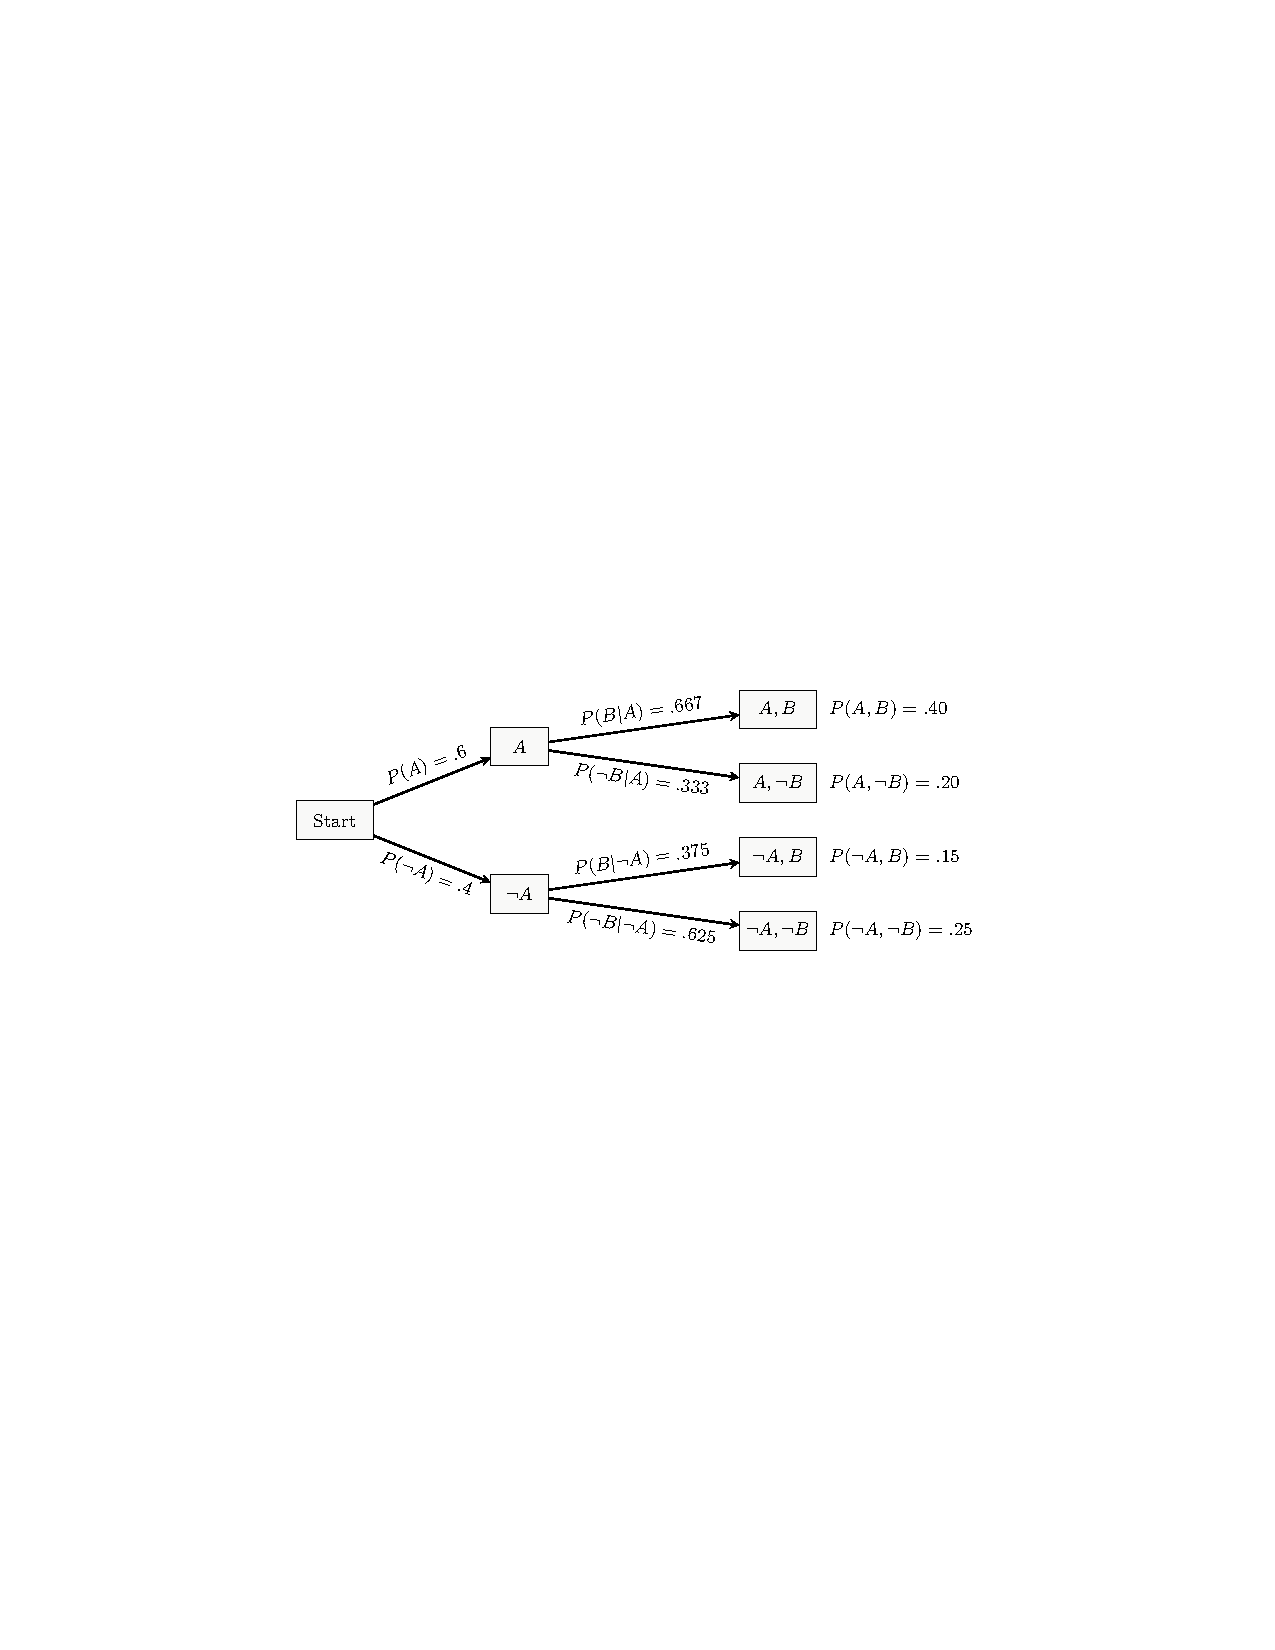
\includegraphics[scale=1,viewport=142 335 466 461]{figs/etzvandekerckhove_fig1.pdf}
\end{center}
\caption{An illustration of the Product Rule of probability: The probability of the joint events on the right end of the diagram is obtained by multiplying the probabilities along the path that leads to it. The paths indicate where and how we are progressively splitting the initial probability into smaller subsets.  A suggested exercise to test understanding and gain familiarity with the rules is to construct the equivalent path diagram (i.e., that in which the joint probabilities are identical) starting on the left with a fork that depends on the event $B$ instead of $A$.}
\label{fig:path}
\end{figure*}

In the next section, we will introduce the basic rules of probability theory. These rules are agnostic to our conception of probability---they hold equally for epistemic and aleatory probability---but throughout the rest of this paper and particularly in the examples, we will, unless otherwise noted, use an epistemic interpretation of the word ``probability.''

\subsection*{The Product and Sum Rules of Probability}
Here we will introduce the two cardinal rules of probability theory from which essentially all of Bayesian inference derives. However, before we venture into the laws of probability, there are notational conventions to draw. First, we will use $P(A)$ to denote the probability of some event $A$, where $A$ is a statement that can be true or false (e.g., $A$ could be ``it will rain today'', ``the UK will be outside the EU on December 31, 2018'', or ``the \nth{20} digit of $\pi$ is 3''). Next, we will use $(B|A)$ to denote the \emph{conditional} event: the probability that {$B$} is true \emph{given that $A$ is true} (e.g., $B$ could be ``it will rain tomorrow'') is $P(B|A)$: the probability that it will rain tomorrow given that it rained today.  Third, we will use $(A,B)$ to denote a \emph{joint} event: the probability that $A$ and $B$ are both true is $P(A,B)$. The joint probability $P(A,B)$ is of course equal to that of the joint probability $P(B,A)$: the event ``it rains tomorrow and today'' is logically the same as ``it rains today and tomorrow.'' Finally, we will use $(\neg A)$ to refer to the negation of $A$: the probability $A$ is false is $P(\neg A)$. These notations can be combined: if $C$ and $D$ represent the events ``it is hurricane season'' and ``it rained yesterday,'' respectively, then $P(A,B|\neg C,\neg D)$ is the probability that it rains today and tomorrow, given that ($\neg C$) it is not hurricane season and that ($\neg D$) it did not rain yesterday (i.e., both $C$ and $D$ are not true).

With this notation in mind, we introduce the \textbf{Product Rule of Probability}:
\begin{equation}
\begin{array}{rcl}
P(A,B) &=& P(B)P(A|B)\\ 
&=& P(A)P(B|A).
\end{array}
\label{eq:prodrule}
\end{equation}
In words: the probability that $A$ and $B$ are both true is equal to the probability of $B$ multiplied by the conditional probability of $A$ \textit{assuming $B$ is true}.  Due to symmetry, this is also equal to the probability of $A$ multiplied by the conditional probability of $B$ \textit{assuming $A$ is true}. The probability it rains today and tomorrow is the probability it first rains today multiplied by the probability it rains tomorrow \textit{given that we know it rained today}.

If we assume $A$ and $B$ are statistically independent then $P(B)$ equals $P(B|A)$, since knowing $A$ happens tells us nothing about the chance $B$ happens. In such cases, the product rule simplifies as follows:
\begin{equation}
P(A,B) = P(A)P(B|A) = P(A)P(B).
\label{eq:indep}
\end{equation}
Keeping with our example, this would mean calculating the probability it rains both today and tomorrow in such a way that knowledge of whether or not it rained today has no bearing on how strongly we should believe it will rain tomorrow.

Understanding the \textbf{Sum Rule of Probability} requires one further concept: the \emph{disjoint set}.  A disjoint set is nothing more than a collection of mutually exclusive events. To simplify the exposition, we will also assume that exactly one of these events must be true although that is not part of the common definition of such a set. The simplest example of a disjoint set is some event and its denial:\footnote{We use curly braces \{\ldots\} to indicate a set of events. Other common examples of disjoint sets are the possible outcomes of a coin flip: $\{$heads, tails$\}$, or the possible outcomes of a roll of a six-sided die: $\{1, 2, 3, 4, 5, 6\}$. A particularly useful example is the truth of some model $\H$, which must be either true or false: $\{\H, \neg{\H}\}$.} $\{B, \neg{B}\}$. If $B$ represents the event ``It will rain tomorrow,'' then $\neg{B}$ represents the event ``It will not rain tomorrow.'' One and only one of these events must occur, so together they form a disjoint set. If $A$ represents the event ``It will rain today,'' and $\neg{A}$ represents ``It will not rain today'' (another disjoint set), then there are four possible pairs of these events, one of which must be true: $(A,B)$, $(A,\neg{B})$, $(\neg{A},B)$, and $(\neg{A},\neg{B})$. The probability of a single one of the singular events, say $B$, can be found by adding up the probabilities of all of the joint events that contain $B$ as follows: $${P(B) = P(A,B) + P(\neg A, B)}.$$ In words, the probability that it rains tomorrow is the sum of two joint probabilities: (1) the probability it rains today and tomorrow, and (2) the probability it does not rain today but does rain tomorrow. 

In general, if $\{A_1, A_2, \ldots, A_K\}$ is a disjoint set, the Sum Rule of Probability states:
\begin{equation}
\begin{array}{rcl}
P(B) &=&P(A_1,B)+P(A_2,B)+\ldots+P(A_K,B)\\ &=&\displaystyle\sum_{k=1}^K P(A_K,B).
\label{eq:sumrule}
\end{array}
\end{equation}
That is, to find the probability of event $B$ alone you add up all the joint probabilities that involve both $B$ and one element of a disjoint set. Intuitively, it is clear that if one of $\{A_1, A_2, \ldots, A_K\}$ \emph{must} be true, then the probability that \emph{one of these and $B$} is true is equal to the base probability that $B$ is true. 

In the context of empirical data collection, the disjoint set of possible outcomes is often called the \emph{sample space}.

\textbf{An illustration of the Product Rule of Probability} is shown by the path diagram in Figure~\ref{fig:path}. Every fork indicates the start of a disjoint set, with each of the elements of that set represented by the branches extending out. The lines indicate the probability of selecting each element from within the set. Starting from the left, one can trace this diagram to find the joint probability of, say, $A$ and $B$. At the \emph{Start} fork there is a probability of .6 of going along the top arrow to event $A$ (a similar diagram could of course be drawn that starts with $B$): The probability it rains today is .6. Then there is a probability of .667 of going along the next top fork to event $(A,B)$: The probability it rains tomorrow given it rained today is .667. Hence, of the initial .6 probability assigned to $A$, two-thirds of it forks into $(A,B)$, so the probability of $(A,B)$ is $.6 \times .667 = .40$: Given that it rained today, the probability it rains tomorrow is $.667$, so the probability it rains both today \textit{and} tomorrow is .4. The probability of any joint event at the end of a path can be found by multiplying the probabilities of all the forks it takes to get there.

\textbf{An illustration of the Sum Rule of Probability} is shown in Table~\ref{tab:prob}, which tabulates the probabilities of all the joint events found through Figure~\ref{fig:path} in the main cells. For example, adding up all of the joint probabilities across the row denoted $A$ gives $P(A)$. Adding up all of the joint probabilities down the column denoted $B$ gives $P(B)$. This can also be seen by noting that in Figure~\ref{fig:path}, the probabilities of the two child forks leaving from $A$, namely $(A,B)$ and $(A,\neg B)$, add up to the probability indicated in the initial fork leading to $A$. This is true for any value of $P(B|A)$ (and $P(\neg B|A) = 1 - P(B|A)$).

\begin{table}[bt]
\caption{The event $A$ is that it rains today. The event $B$ is that it rains tomorrow. Sum across rows to find $P(A)$, sum down columns to find $P(B)$. One can also divide $P(A,B)$ by $P(A)$ to find $P(B|A)$, as shown in the next section.}
\label{tab:prob}\centering
\begin{tabular}{cr@{ = }lr@{ = }lcr@{ = }l}
 & \multicolumn{2}{c}{$B$} & \multicolumn{2}{c}{$\neg{B}$} & &\multicolumn{2}{c}{$B$ \textit{or} $\neg{B}$}
 \\[0.5ex]
\hline
$A$ & $P(A,B)$ & $.40$ & $P(A,\neg{B})$ & $.20$ & $\Rightarrow$ & $P(A)$ & $.60$\\
$\neg{A}$ & $P(\neg{A},B)$ & $.15$ & $P(\neg{A},\neg{B})$ & $.25$ & $\Rightarrow$ & $P(\neg A)$ & $.40$ \\[0.5ex] 
$A$ \textit{or} $\neg A$ & $P(B)$ & $.55$ & $P(\neg B)$ & $.45$ && \multicolumn{2}{c}{$1.00$} \\[0.5ex]\hline
\end{tabular}
\end{table}
 
\section*{What is Bayesian inference?}
\epigraph{Together [the Sum and Product Rules] solve the problem of inference, or, better, they provide a framework for its solution.}{D.~V.~\citeA{Lindley2000}}

\noindent \textbf{Bayesian inference is the application of the product and sum rules to real problems of inference}. Applications of Bayesian inference are creative ways of looking at a problem through the lens of these two rules. The rules form the basis of a mature philosophy of scientific learning {proposed} by Dorothy Wrinch and Sir Harold Jeffreys  (\citeNP{Jeffreys1961,Jeffreys1973,WrinchJeffreys1921}; see also \citeNP{LyEtAl2016}). Together, the two rules allow us to calculate probabilities and perform scientific inference in an incredible variety of circumstances. We begin by illustrating one combination of the two rules that is especially useful for scientific inference: Bayesian hypothesis testing.

\subsection*{Bayes' Rule}
Call event $\H$ (the truth of) an hypothesis that a researcher holds and call $\neg{\H}$ a competing hypothesis. 
Together these {can} form a disjoint set: $\{\H,\neg{\H}\}$. The set $\{\H,\neg{\H}\}$ is necessarily disjoint if $\neg{\H}$ is simply the denial of $\H$, but in practice the set of hypotheses can contain any number of models spanning a wide range of theoretical accounts. In such a scenario, it is important to keep in mind that we cannot make inferential statements about any model not included in the set.

Before any data are collected, the researcher has some level of prior belief in these competing hypotheses, which manifest as \textit{prior probabilities} and are denoted $P(\H)$ and $P(\neg{\H})$. The hypotheses are well-defined if they make a specific prediction about the probability of each experimental outcome $X$ through the \emph{likelihood functions} $P(X|\H)$ and $P(X|\neg\H)$. Likelihoods can be thought of as how strongly the data $X$ are implied by an hypothesis. \textit{Conditional} on the truth of an hypothesis, likelihood functions specify the probability of a given outcome and are usually easiest to interpret in relation to other hypotheses' likelihoods. Of interest, of course, is the probability that $\H$ is true, given the data $X$, or $P(\H|X)$. 

By simple rearrangement of the factors of the Product Rule shown in the first line of Equation~\ref{eq:prodrule}, $P(\H,X)=P(X)P(\H|X)$, we can derive that $$P(\H|X) = \frac{P(\H,X)}{P(X)}.$$  Due to the symmetric nature of the Product Rule, we can reformulate the joint event in the numerator above by applying the product rule again as in the second line in Equation~\ref{eq:prodrule}, $P(\H,X)=P(\H)P(X|\H)$, and we see that this is equivalent to
\begin{equation}
P(\H|X) = \frac{P(\H)P(X|\H)}{P(X)}.
\label{eq:bayesrule}
\end{equation}
Equation~\ref{eq:bayesrule} is one common formulation of \textbf{Bayes' Rule}, and analogous versions can be written for each of the other competing hypotheses; for example, Bayes' Rule for $\neg\H$ is $$P(\neg\H|X) = \frac{P(\neg\H)P(X|\neg\H)}{P(X)}.$$ The probability of an hypothesis given the data is equal to the probability of the hypothesis before seeing the data, multiplied by the probability that the data occur if that hypothesis is true, divided by the prior predictive probability of the observed data (see below). In the way that $P(\H)$ and $P(\neg\H)$ are called prior probabilities because they capture our knowledge prior to seeing the data $X$, so $P(\H|X)$ and $P(\neg\H|X)$ are called the \emph{posterior probabilities}. 

\subsection*{The prior predictive probability $P(X)$}
Many of the quantities in Equation~\ref{eq:bayesrule} we know: we must have some prior probability (belief or prior information) that the hypothesis is true if we are even considering the hypothesis at all, and if the hypothesis is well-described it will attach a particular probability to the observed data. What remains is the denominator: the prior predictive probability $P(X)$---the probability of observing a given outcome in the experiment, which can be thought of as the average probability of the outcome implied by the hypotheses, weighted by the prior probability of each hypothesis. $P(X)$ can be obtained through the sum rule by adding the probabilities of the joint events $P(X,\H)$ and $P(X,\neg{\H})$, as in Equation~\ref{eq:sumrule}, each of which is obtained through an application of the product rule, so we obtain the following expression:
\begin{equation}\label{eq:marginal}\begin{array}{rcl}
P(X) &=& P(X,\H) + P(X,\neg{\H})\\ 
&=& P(\H)P(X|\H) + P(\neg{\H})P(X|\neg{\H}),
\end{array}\end{equation}
which amounts to adding up the right-hand side numerator of Bayes' Rule for all competing hypotheses, giving a weighted-average probability of observing the outcome $X$. 

Now that we have a way to compute $P(X)$ in Equation~\ref{eq:marginal}, we can plug the result into the denominator of Equation~\ref{eq:bayesrule} as follows: \begin{equation}\label{eq:bayesrule1}P(\H|X) = \frac{P(\H)P(X|\H)}{P(\H)P(X|\H) + P(\neg{\H})P(X|\neg{\H})}.\end{equation}

Equation~\ref{eq:bayesrule1} is for the case where we are only considering one hypothesis and its complement. More generally,
\begin{equation}
P(\H_i|X) = \frac{P(\H_i)P(X|\H_i)}{\sum_{k=1}^K P(\H_k)P(X|\H_k)},
\label{eq:bayesrule2}
\end{equation}
for the case where we are considering $K$ competing and mutually-exclusive hypotheses (i.e., hypotheses that form a disjoint set), one of which is $\H_i$. 

\subsection*{Quantifying evidence}
Now that we have, in one equation, factors that correspond to our knowledge before---$P(\H)$---and after---$P(\H|X)$---seeing the data, we can address a slightly alternative question: \emph{How much did we learn due to the data $X$?} Consider that every quantity in Equation~\ref{eq:bayesrule2} is either a prior belief in an hypothesis, or the probability that the data would occur under a certain hypothesis---all known quantities. If we divide both sides of Equation~\ref{eq:bayesrule2} by $P(\H_i)$,
\begin{eqnarray}
\frac{P(\H_i|X)}{P(\H_i)} = \frac{P(X|\H_i)}{\sum_{k=1}^K P(\H_k)P(X|\H_k)},
\end{eqnarray}
we see that after observing outcome $X$, the ratio of an hypothesis's posterior probability to its prior probability is larger than 1 (i.e., its probability goes up) if {the probability it attaches to the observed outcome is greater than a weighted-average of all such probabilities -- averaged across all candidate hypotheses, using the respective prior probabilities as weights.}

If we are concerned with only two hypotheses, a particularly interesting application of Bayes' Rule becomes possible. After collecting data we are left with the posterior probability of two hypotheses, $P(\H|X)$ and $P(\neg\H|X)$. If we form a ratio of these probabilities we can quantify our \emph{relative belief} in one hypothesis vis-\`a-vis the other, or what is known as the posterior odds: $P(\H|X)/P(\neg\H|X)$. If $P(\H|X) = .75$ and $P(\neg\H|X) = .25$, the posterior odds are $.75/.25 = 3$, or \odds{3}{1} (``three to one'') in favor of $\H$ over $\neg\H$. Since the posterior probability of an hypothesis is equal to the fraction in the right-hand side of Equation~\ref{eq:bayesrule1}, we can calculate the posterior odds as a ratio of two right-hand sides of Bayes' Rule as follows: $$ \dfrac{P(\H|X)}{P(\neg\H|X)} = \dfrac{\,\,\,\dfrac{P(\H)P(X|\H)}{P(\H)P(X|\H) + P(\neg{\H})P(X|\neg{\H})}\,\,\,}{\dfrac{P(\neg\H)P(X|\neg\H)}{P(\H)P(X|\H) + P(\neg{\H})P(X|\neg{\H})}}, $$ which can be reduced to a simple expression (since the denominators cancel out),
\begin{equation}
\underbrace{\frac{P(\H|X)} {P(\neg\H|X)}}_\text{Posterior odds} =
\underbrace{\frac{P(\H)}{P(\neg\H)}}_\text{Prior odds} \ \times \
\underbrace{\frac{P(X|\H)}{P(X|\neg\H)}}_\text{Bayes factor}.\label{eq:bayesodds}
\end{equation}
The final factor---the Bayes factor---can be interpreted as \emph{the extent to which the data sway our relative belief from one hypothesis to the other}, which is determined by comparing the hypotheses' abilities to predict the observed data. If the data are more probable under $\H$ than under $\neg \H$ (i.e., if $P(X|\H)$ is larger than $P(X|\neg \H)$) then $\H$ does the better job predicting the data, and the posterior odds will favor $\H$ more strongly than the prior odds.

It is important to distinguish Bayes factors from posterior probabilities. Both are useful in their own role -- posterior probabilities to determine our total belief after taking into account the data and to draw conclusions, and Bayes factors as a learning factor that tells us how much evidence the data have delivered. It is often the case that a Bayes factor favors $\H$ over $\neg\H$ while at the same time the posterior probability of $\neg\H$ remains greater than $\H$.  As Jeffreys, in his seminal paper introducing the Bayes factor as a method of inference, explains: ``If \dots  the [effect] examined is one that previous considerations make unlikely to exist, then we are entitled to ask for a greater increase of the probability before we accept it,'' and moreover, ``To raise the probability of a proposition from 0.01 to 0.1 does not make it the most likely alternative'' \cite[p.\ 221]{Jeffreys1935}. This distinction is especially relevant to today's publishing environment, where there exists an incentive to publish counterintuitive results -- whose very description as counterintuitive implies most researchers would not have expected them to be true. Consider as an extreme example \citeA{Bem2011} who presented data consistent with the hypothesis that some humans can predict future random events. While Bem's data may indeed provide positive evidence for that hypothesis \cite{RouderMorey2011}, it is staggeringly improbable a priori and the evidence in the data does not stack up to the strong priors many of us will have regarding extrasensory perception -- extraordinary claims require extraordinary evidence.

Since Bayes factors quantify statistical evidence, they can serve two (closely related) purposes. First, evidence can be applied to defeat prior odds: supposing that prior to the data we believe that $\neg\H$ is three times more likely than $\H$ (i.e., the prior ratio favoring $\neg\H$ is 3, or its prior probability is 75\%), we need a Bayes factor favoring $\H$ that is greater than 3 so that $\H$ will end up the more likely hypothesis. Second, evidence can be applied to achieve a desired level of certainty: supposing that we desire a high degree of certainty before making any practical decision (say, at least 95\% certainty or a posterior ratio of at least 19) and supposing the same prior ratio as before, then we would require a Bayes factor of $19 \times 3 = 57$ to defeat the prior odds and obtain this high degree of certainty. {These practical considerations (often left implicit) are formalized by utility (loss) functions in \textit{Bayesian decision theory}. We will not go into Bayesian decision theory in depth here; introductions can be found in \citeA{lindley1985} or \citeA{winkler1972book}, and an advanced introduction is available in \citeA{robert2007}.}

In this section, we have derived Bayes' Rule as a necessary consequence of the laws of probability. The rule allows us to update our belief regarding an hypothesis in response to data. Our beliefs after taking account the data are captured in the \emph{posterior probability}, and the amount of updating is given by the \emph{Bayes factor}.  We now move to some applied examples that illustrate how this simple rule pertains to cases of inference.

\example{Frontier xenobotanist} At the Resistance base on Ajan Kloss,\footnote{With our apologies to George Lucas.} Rey tends a small xenobotanical laboratory {(see Illustration)}. In a humid enclosure assembled from salvaged starship parts, she cultivates crops of a local plant called the \emph{green glowcap} -- a flowering organism that, when consumed, causes most humanoids to feel euphoric and relaxed. Finn is an enthusiastic consumer of green glowcap and frequently visits Rey's laboratory to sample the latest harvest.

\begin{figure}[tb]
\centering
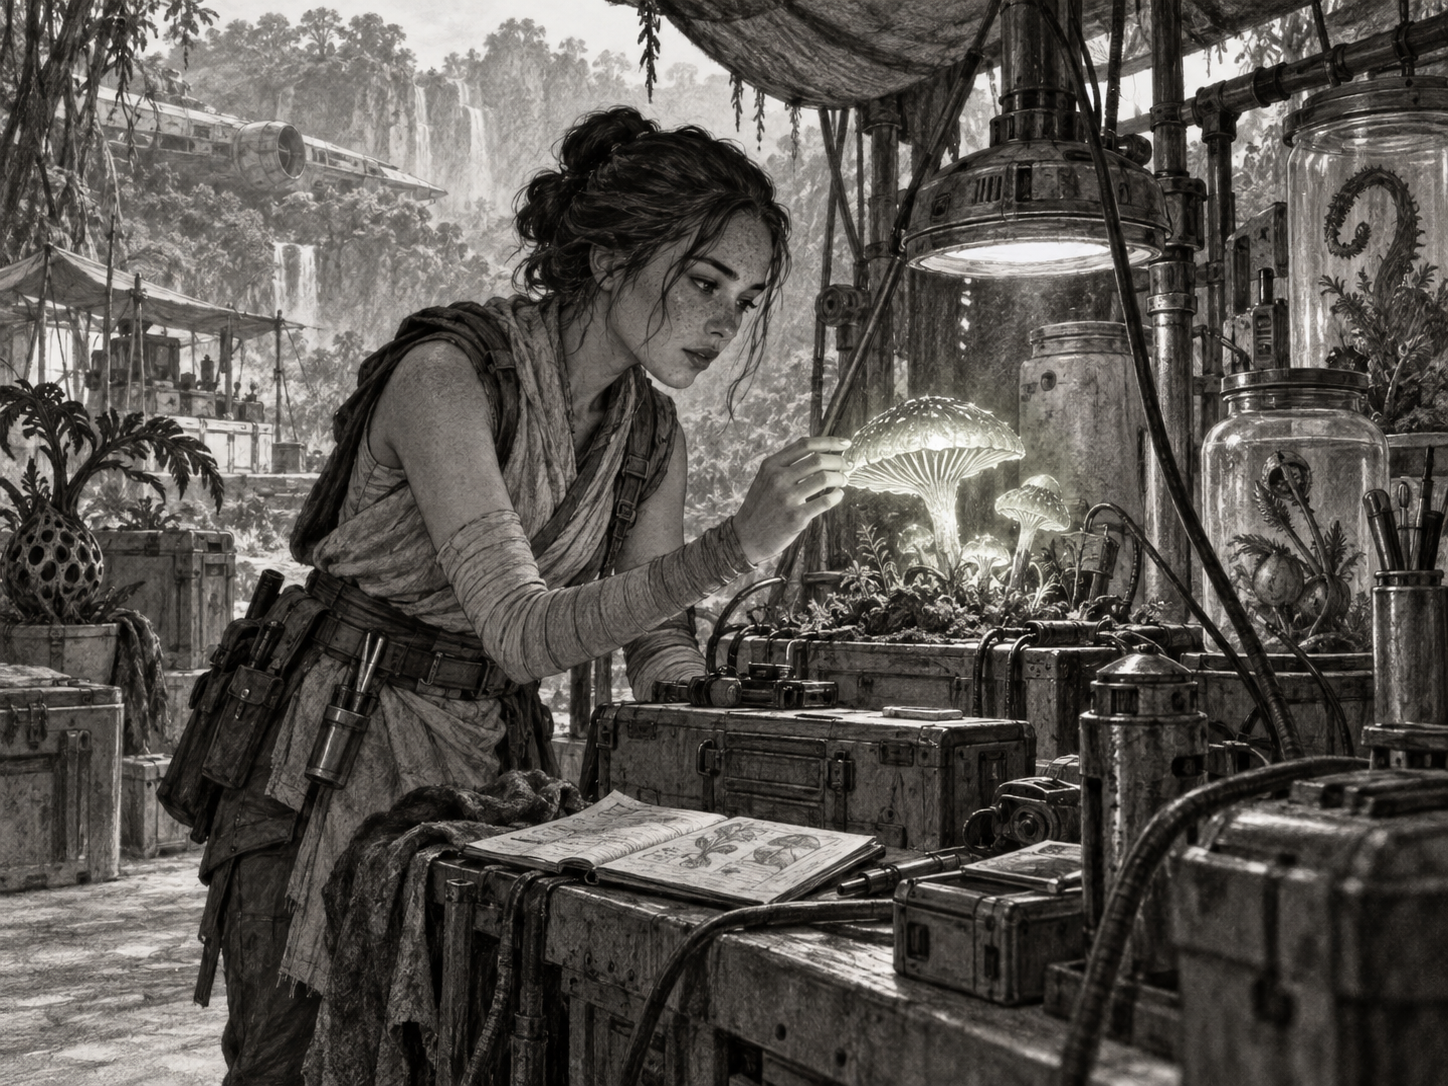
\includegraphics[width=.47\textwidth]{figs/starwars_illustration.png}
\caption*{\textit{Illustration.} Rey examines a green glowcap in her improvised xenobotanical laboratory on Ajan Kloss.}\label{ill:glowcap}
\end{figure}

However, it has turned out that one in a thousand glowcaps is afflicted with a mutation that changes its effects: Consuming those rare plants causes unpleasant side effects such as paranoia, anxiety, and brief, uncontrolled sensitivity to the Force. In order to evaluate the quality of her crops, Rey has assembled a mutation-detecting bioscanner. The new scanner has a 99\% chance to accurately detect an existing mutation, but also {has a 2\% chance to} falsely indicate that a healthy plant is a mutant. When Rey mentions her findings, Finn asks two questions: What is the probability that a glowcap is a mutant, when your scanner says that it is? And what is the probability the plant is a mutant, when your scanner says that it is healthy? Finn's interest is in knowing how much trust to put into Rey's scanner before taking another sample.

\begin{figure*}[tbhp]
\begin{center}
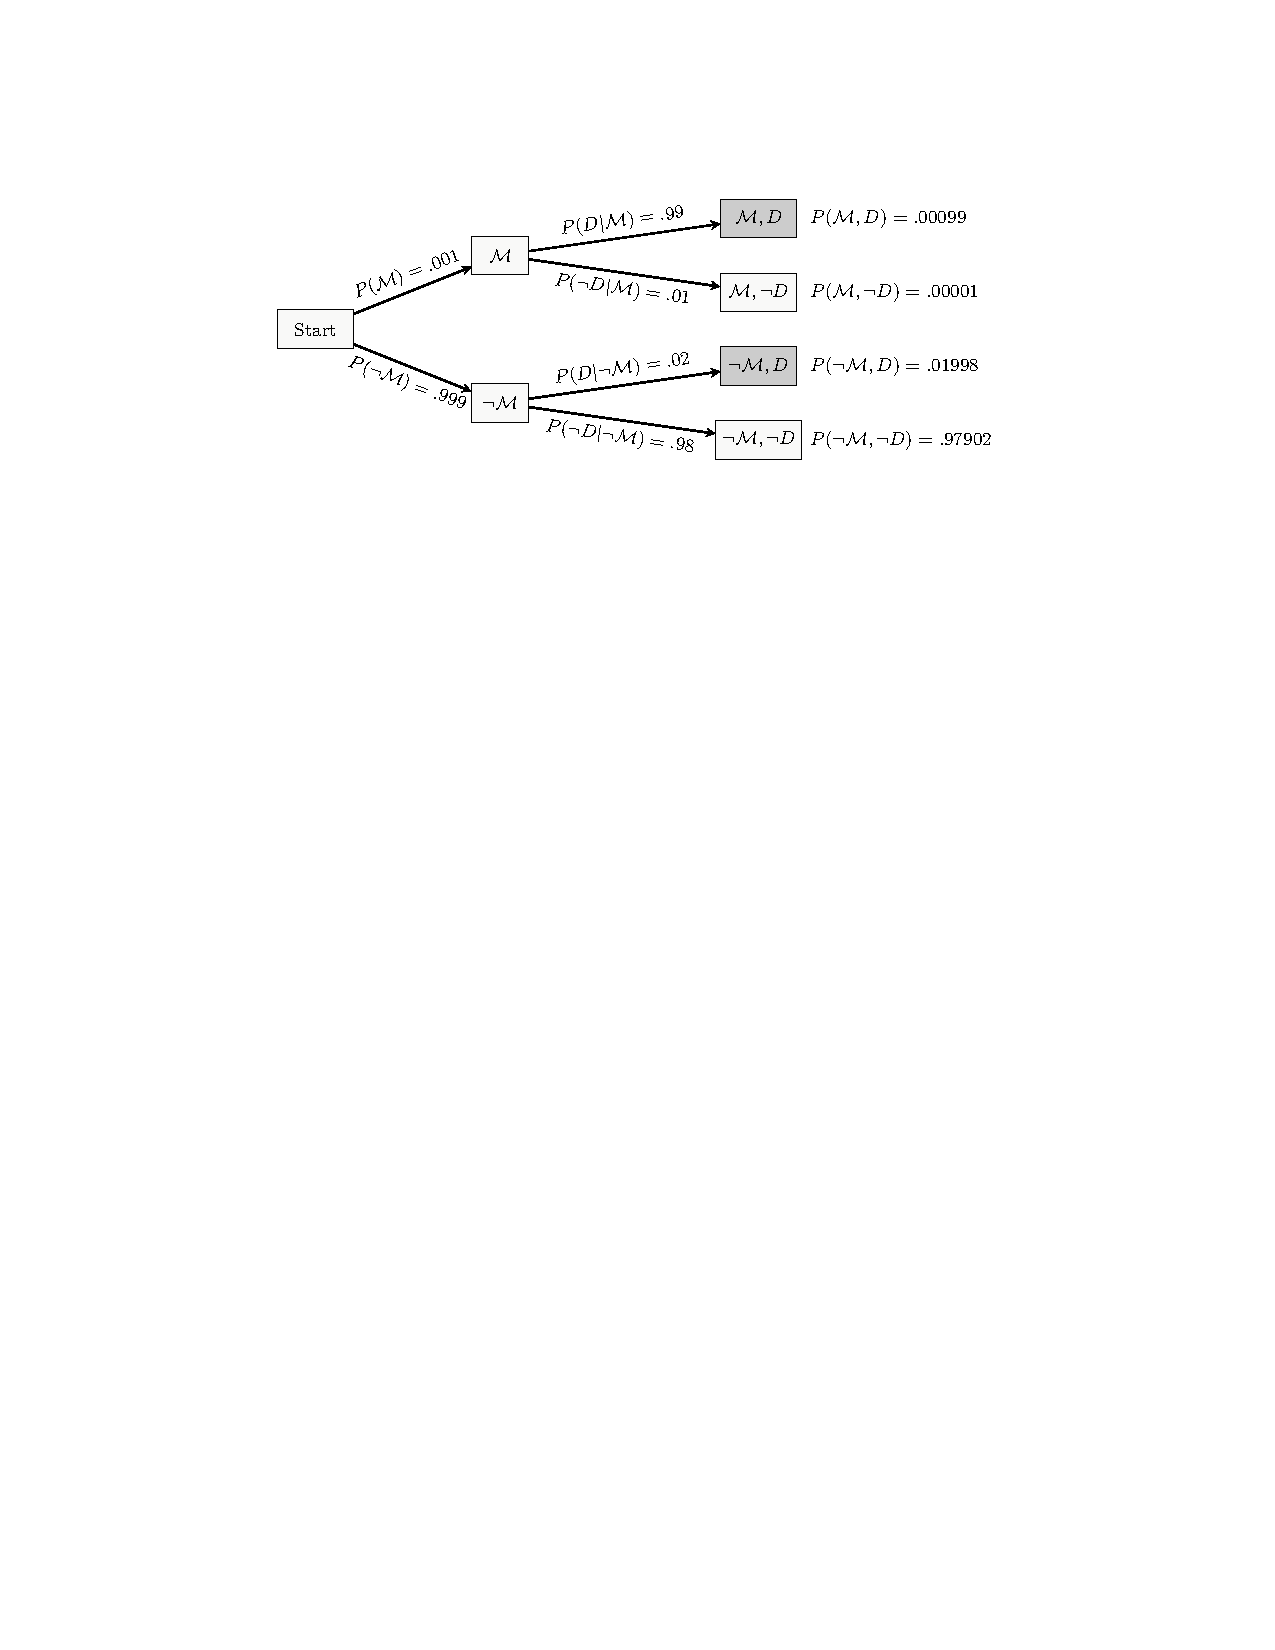
\includegraphics[scale=1,viewport=133 571 475 696]
{figs/etzvandekerckhove_fig2.pdf}
\end{center}
\caption{The event $\H$ is that a given glowcap is a mutant. The event $D$ is that Rey's bioscanner returns a mutant diagnosis. A mutant diagnosis $D$ is in fact observed, so the only paths that remain relevant are those that lead to a mutant diagnosis (events $(\H,D)$ and $(\neg\H,D)$, shaded). Finn takes the following steps to find the posterior probability the plant is a mutant given the mutant diagnosis: Multiply $P(\H)$ by $P(D|\H)$ to find $P(\H,D)$; multiply $P(\neg \H)$ by $P(D|\neg \H)$ to find $P(\neg \H,D)$; add $P(\H,D)$ and $P(\neg \H, D)$ to find $P(D)$; divide $P(\H,D)$ by $P(D)$ to find $P(\H|D)$. Finn's question can be rephrased as: of the total probability remaining in the diagram after $D$ is observed -- which is equal to $P(D)$ -- what proportion of it originated at the $\H$ node? The results of Finn's calculations are given in the text.}
\label{fig:codacle}
\end{figure*}

Call the event that a specific plant is a mutant $\H$, and that it is healthy $\neg \H$. Call the event that Rey's bioscanner diagnoses a plant as a mutant $D$, and that it diagnoses it healthy $\neg D$. Finn's interest is in the probability that the plant is indeed a mutant given that it has been diagnosed as a mutant, or $P(\H|D)$, and the probability the plant is a mutant given it has been diagnosed healthy, or $P(\H|\neg D)$. Finn, who learned to respect unfavorable odds while serving in the First Order, has all the relevant information to apply Bayes' Rule (Equation~\ref{eq:bayesrule2} above) to find these probabilities. He knows the prior probability that a plant is a mutant is $P(\H) = .001$, and thus the prior probability that a plant is not a mutant is $P(\neg \H) = 1 - P(\H) = .999$. The probability of a correct mutant diagnosis given the plant is a mutant is $P(D|\H) = .99$, and the probability of an erroneous healthy diagnosis given the plant is a mutant is thus $P(\neg D|\H) = 1 - P(D|\H) = .01$. When the plant is healthy, the scanner incorrectly diagnoses it as a mutant with probability $P(D|\neg \H) = .02$, and correctly diagnoses the plant as healthy with probability $P(\neg D|\neg \H) = 1 - P(D|\neg \H) = .98$.

When Rey's scanner gives a mutant diagnosis, the posterior probability that the plant is really a mutant is given by Bayes' Rule: $$P(\H|D) = \frac{P(\H)P(D|\H)}{P(\H)P(D|\H) + P(\neg \H)P(D|\neg \H)}.$$ Finn can now consult Figure~\ref{fig:codacle} to find that the posterior probability the plant is a mutant given a mutant diagnosis is: $$P(\H|D) = \frac{.001 \times .99}{.001 \times .99 + .999\times .02} \approx .047.$$ A mutant diagnosis from Rey's scanner raises the probability the plant is a mutant from $.001$ to roughly $.047$. This means that when a plant is diagnosed as a mutant, the posterior probability the plant is \textit{not} a mutant is $P(\neg \H|D) \approx 1 - .047 = .953$. The low prior probability that a plant is a mutant means that, even with the scanner having 99\% accuracy to correctly diagnose a mutant plant as such, a plant diagnosed as a mutant is still probably safe to eat -- nevertheless, Finn will think twice.

Analogous calculations show that the posterior probability that a plant is a dangerous mutant, given it is diagnosed as healthy, is: $$P(\H|\neg D) = \frac{.001 \times .01}{.001 \times .01 + .999\times .98} \approx .000010.$$ The posterior probability that a plant is a dangerous mutant despite being diagnosed as healthy is quite small, so Finn can be relatively confident he is eating a healthy plant after Rey's scanner returns a healthy diagnosis.

A major advantage of using Bayes' Rule in this way is that it gracefully extends to more complex scenarios. Consider the perhaps disappointing value of $P(\H|D)$: a mutant diagnosis only raises the posterior probability to just under 5\%. Suppose, however, that Finn knows that the diagnosis from Rey's field sensor ($D_S$) is statistically independent from the diagnosis produced by Rose Tico's {carefully calibrated} laboratory analyzer ($D_L$) -- meaning that for any given state of nature $\H$ or $\neg{\H}$, the laboratory diagnosis does not depend on the sensor diagnosis. Further suppose that both devices return the mutant diagnosis (and for simplicity we also assume Rose's analyzer is equally as accurate as Rey's sensor). To find the posterior probability the plant is a mutant after two independent mutant diagnoses, $P(\H|D_S, D_L)$, Finn can apply a fundamental principle in Bayesian inference: \textbf{Yesterday's posterior is today's prior} {\cite{Lindley2000}}.

Since we take diagnosis $D_S$ and diagnosis $D_L$ as conditionally independent, we know that $P(D_L|\H,D_S)=P(D_L|\H)$ and $P(D_L|\neg \H,D_S)=P(D_L|\neg \H)$, giving
\begin{multline*}
P(\H|D_S, D_L) \\
= \frac{P(\H|D_S)P(D_L|\H)}{P(\H|D_S)P(D_L|\H) + P(\neg \H|D_S)P(D_L|\neg \H)} \\
= \frac{.047 \times .99}{.047 \times .99 + .953\times .02} \approx .71,
\end{multline*}
where the probability the plant is a mutant \textit{prior to the laboratory diagnosis $D_L$}, $P(\H|D_S)$, is the probability it is a mutant \textit{posterior to the sensor diagnosis $D_S$}. This illustrates the value of multiple independent sources of evidence: a plant that has twice been independently diagnosed as a mutant is quite likely to be one. A third independent diagnosis would put the posterior probability over 99\%. {Note that, crucially, we would have obtained precisely the same final probability of $.71$ had we updated $P(\H)$ to $P(\H|D_S,D_L)$ all at once. This is easily confirmed when we consider the two diagnoses as a joint event $(D_S,D_L)$ and use the conditional probability $P(D_S,D_L|\H) = P(D_S | \H) \times P(D_L | \H)$ (as in Equation~\ref{eq:indep}) to update $P(\H)$ to $P(\H|D_S,D_L)$ in a single step.}

\paragraph{Discussion} 
It is instructive to consider some parallels of this (admittedly fictional) example to current practices in social science. The scenario is similar in setup to a null-hypothesis significance testing scenario in which one defines the null hypothesis $\mathcal{H}_0$ (e.g., that there is no effect of some manipulation) and its negation $\mathcal{H}_1$ (that there is an effect), and the end goal is to make a choice between two possible decisions $\{D,\neg D\}$; $D$ means deciding to reject $\mathcal{H}_0$, and $\neg D$ means deciding not to reject $\mathcal{H}_0$. In the example above the rate at which we falsely reject the null hypothesis (i.e., deciding to reject it when in fact it is true) is given by $P(D|\neg\H) = .02$ -- this is what is commonly called the false alarm rate. The rate at which we correctly reject the null hypothesis (i.e., rejecting it if it is false) is $P(D|\H) = .99$. However, even with a low false alarm rate and a very high correct rejection rate, a null hypothesis rejection may not necessarily provide enough evidence to overcome the low prior probability an alternative hypothesis might have.


\example{The phantom assignment}\label{ex:assign}
At the start of every training cycle, new Resistance recruits are assigned to one of four service tracks: Gunnery, Heavy Weapons, Reconnaissance, or Starfighter Operations. The assignment is performed by an ancient allocation droid that analyzes each recruit's abilities and temperament before announcing the track that it determines to be the best fit. For eons the droid has assigned troops with perfect accuracy and in perfect balance (one-quarter to each track).

Unfortunately, the droid was struck by a stray blaster bolt during an evacuation. As a result of the damage, it will now occasionally announce ``Starfighter Operations!'' even when a recruit's proper assignment is elsewhere. Now, the droid places exactly 40\% of recruits in Starfighter Operations instead of the usual 25\%, and each of the other tracks gets only 20\% of the cohort.

To correct the assignments, C3PO considers an alternative written test---the \emph{Placement Aptitude Review for Service Expertise and Classification} or P.A.R.S.E.C.\ test---on which true Starfighter recruits will tend to score \emph{Excellent} ($S_E$), while Reconnaissance recruits will tend to score \emph{Outstanding} ($S_O$), Gunnery recruits \emph{Acceptable} ($S_A$), and Heavy Weapons recruits \emph{Poor} ($S_P$). Benchmark tests on recruits assigned before the droid was damaged have revealed the approximate distribution of P.A.R.S.E.C.\ scores within each track (see Table~\ref{tab:sorting}). The test is administered to all recruits whom the damaged droid assigns to Starfighter Operations, and their score determines the track to which they are ultimately assigned. C3PO is now asked to determine the probability that a recruit assigned to Starfighter Operations who scored \emph{Excellent} on the P.A.R.S.E.C.\ test actually belongs in Gunnery.

\FPset{\pes}{0.80} \FPset{\pos}{0.10} \FPset{\pas}{0.05} \FPset{\pps}{0.05}  
\FPset{\peg}{0.05} \FPset{\pog}{0.20} \FPset{\pag}{0.70} \FPset{\ppg}{0.05}  
\FPset{\per}{0.05} \FPset{\por}{0.80} \FPset{\parr}{.15} \FPset{\ppr}{0.00}  
\FPset{\peh}{0.00} \FPset{\poh}{0.10} \FPset{\pah}{0.25} \FPset{\pph}{0.65}  

\FPset{\pss}{1.00} \FPset{\ps}{0.25}  
\FPset{\psg}{0.20} \FPset{\pg}{0.25}  
\FPset{\psr}{0.20} \FPset{\pr}{0.25}  
\FPset{\psh}{0.20} \FPset{\ph}{0.25}  

\FPeval{\jsse} {\ps*\pes*\pss}  % P(S,S,E)
\FPeval{\jgse} {\pg*\peg*\psg}  % P(G,S,E)
\FPeval{\jrse} {\pr*\per*\psr}  % P(R,S,E)
\FPeval{\jhse} {\ph*\peh*\psh}  % P(H,S,E)
\FPeval{\jsso} {\ps*\pos*\pss}  % P(S,S,O)
\FPeval{\jgso} {\pg*\pog*\psg}  % P(G,S,O)
\FPeval{\jrso} {\pr*\por*\psr}  % P(R,S,O)
\FPeval{\jhso} {\ph*\poh*\psh}  % P(H,S,O)
\FPeval{\jssa} {\ps*\pas*\pss}  % P(S,S,A)
\FPeval{\jgsa} {\pg*\pag*\psg}  % P(G,S,A)
\FPeval{\jrsa} {\pr*\parr*\psr} % P(R,S,A)
\FPeval{\jhsa} {\ph*\pah*\psh}  % P(H,S,A)
\FPeval{\jssp} {\ps*\pps*\pss}  % P(S,S,P)
\FPeval{\jgsp} {\pg*\ppg*\psg}  % P(G,S,P)
\FPeval{\jrsp} {\pr*\ppr*\psr}  % P(R,S,P)
\FPeval{\jhsp} {\ph*\pph*\psh}  % P(H,S,P)

\FPeval{\pse} {\jsse + \jgse + \jrse + \jhse}  % P(S,E)
\FPeval{\pso} {\jsso + \jgso + \jrso + \jhso}  % P(S,O)
\FPeval{\psa} {\jssa + \jgsa + \jrsa + \jhsa}  % P(S,A)
\FPeval{\psp} {\jssp + \jgsp + \jrsp + \jhsp}  % P(S,P)

\FPeval{\psse} {\jsse/\pse} \FPeval{\pssepct}{100*\psse} % P(S|S,E)
\FPeval{\pgse} {\jgse/\pse} \FPeval{\pgsepct}{100*\pgse} % P(G|S,E)
\FPeval{\prse} {\jrse/\pse} \FPeval{\prsepct}{100*\prse} % P(R|S,E)
\FPeval{\phse} {\jhse/\pse} \FPeval{\phsepct}{100*\phse} % P(H|S,E)
\FPeval{\psso} {\jsso/\pso} \FPeval{\pssopct}{100*\psso} % P(S|S,O)
\FPeval{\pgso} {\jgso/\pso} \FPeval{\pgsopct}{100*\pgso} % P(G|S,O)
\FPeval{\prso} {\jrso/\pso} \FPeval{\prsopct}{100*\prso} % P(R|S,O)
\FPeval{\phso} {\jhso/\pso} \FPeval{\phsopct}{100*\phso} % P(H|S,O)
\FPeval{\pssa} {\jssa/\psa} \FPeval{\pssapct}{100*\pssa} % P(S|S,A)
\FPeval{\pgsa} {\jgsa/\psa} \FPeval{\pgsapct}{100*\pgsa} % P(G|S,A)
\FPeval{\prsa} {\jrsa/\psa} \FPeval{\prsapct}{100*\prsa} % P(R|S,A)
\FPeval{\phsa} {\jhsa/\psa} \FPeval{\phsapct}{100*\phsa} % P(H|S,A)
\FPeval{\pssp} {\jssp/\psp} \FPeval{\pssppct}{100*\pssp} % P(S|S,P)
\FPeval{\pgsp} {\jgsp/\psp} \FPeval{\pgsppct}{100*\pgsp} % P(G|S,P)
\FPeval{\prsp} {\jrsp/\psp} \FPeval{\prsppct}{100*\prsp} % P(R|S,P)
\FPeval{\phsp} {\jhsp/\psp} \FPeval{\phsppct}{100*\phsp} % P(H|S,P)

\begin{table*}[th]
\caption{Probability of each P.A.R.S.E.C.\ score by true service-track affiliation. {Each value indicates the conditional probability $P(S|\H)$, that is, the probability that a recruit from track $\H$ obtains score $S$.}}
\centering
\begin{tabular}{lccccc}
              & Excellent ($S_E$) & Outstanding ($S_O$) & Acceptable ($S_A$) & Poor ($S_P$) \\ \hline
Starfighter Operations ($\H_S$)&\print[2]{\pes}&\print[2]{\pos}&\print[2]{\pas}&\print[2]{\pps}\\
Gunnery                ($\H_G$)&\print[2]{\peg}&\print[2]{\pog}&\print[2]{\pag}&\print[2]{\ppg}\\
Reconnaissance         ($\H_R$)&\print[2]{\per}&\print[2]{\por}&\print[2]{\parr}&\print[2]{\ppr}\\
Heavy Weapons          ($\H_H$)&\print[2]{\peh}&\print[2]{\poh}&\print[2]{\pah}&\print[2]{\pph}\\
 \hline
\end{tabular}\label{tab:sorting}
\end{table*}

The solution relies on the repeated and judicious application of the Sum and Product Rules, until an expression appears with the desired quantity on the left hand side and only known quantities on the right hand side. To begin, C3PO writes down Bayes' Rule (remembering that a joint event like $(D_S, S_E)$ can be treated like any other event):
$$P(\H_G|D_S,S_E) = \frac{P(\H_G)P(D_S,S_E|\H_G)}{P(D_S,S_E)}$$ Here, $\H_G$ means that the true service-track assignment is Gunnery, $D_S$ means that the allocation droid placed the recruit in Starfighter Operations, and $S_E$ means the recruit scored \emph{Excellent} on the P.A.R.S.E.C.\ test.

In most simple cases, we often have knowledge of simple probabilities, of the form $P(A)$ and $P(B|A)$, while the probabilities of joint events $(A,B)$ are harder to obtain. For C3PO's problem, we can overcome this difficulty by using the Product Rule to unpack the joint event in the numerator:\footnote{Note that this is an application of the Product Rule to the scenario where both events are conditional on $\H_G$: $P(D_S,S_E|\H_G) = P(S_E|\H_G)P(D_S|S_E,\H_G)$.} $$P(\H_G|D_S,S_E) = \frac{P(\H_G)P(S_E|\H_G)P(D_S|S_E,\H_G)}{P(D_S,S_E)}.$$ Now we discover the probability $P(D_S|S_E,\H_G)$ in the numerator. Since the damaged droid's recommendation does not add any information about the P.A.R.S.E.C.\ score above and beyond the recruit's true service-track affiliation (i.e., it is \emph{conditionally independent}; the test score is not entirely independent of the droid's recommendation since the droid is often right about the recruit's correct affiliation and the affiliation influences the test score), we can simplify this conditional probability: $P(D_S|S_E,\H_G) = P(D_S|\H_G)$. Note that the numerator now only contains known quantities: $P(S_E|\H_G)$ can be read off as 0.05 from Table~\ref{tab:sorting}; $P(D_S|\H_G)$ is the probability that a true Gunnery recruit is erroneously assigned to Starfighter Operations, and since that happens to one in five true Gunnery recruits (because the proportion assigned to Gunnery went down from 25\% to 20\%), $P(D_S|\H_G)$ must be 0.20; and $P(\H_G)$ is the base probability that a recruit belongs in Gunnery, which we know to be one in four. Thus,
\begin{eqnarray*}
P(\H_G|D_S,S_E) &=& \frac{P(\H_G)P(S_E|\H_G)P(D_S|\H_G)}{P(D_S,S_E)} \\  
& = & \frac{\print[2]{\pg} \times \print[2]{\peg} \times \print[2]{\psg}}{P(D_S,S_E)}.
\end{eqnarray*}

This leaves us having to find $P(D_S,S_E)$, the prior predictive probability that a recruit would be assigned to Starfighter Operations and score \emph{Excellent} on the P.A.R.S.E.C.\ test. Here, the Sum Rule will help us out, because we can find the right hand side numerator for each type of recruit in the same way we did for true Gunnery recruits above -- we can find $P(D_S,S_E|\H_i)$ for any service track $i = S, G, R, H$. Hence (from Equation~\ref{eq:sumrule}),
\begin{eqnarray*}
P(D_S,S_E)  &=& \sum_i P(\H_i)P(S_E|\H_i)P(D_S|\H_i) \\
 &=&    P(\H_S)P(S_E|\H_S)P(D_S|\H_S) \\
 && {}+ P(\H_G)P(S_E|\H_G)P(D_S|\H_G)\\
 && {}+ P(\H_R)P(S_E|\H_R)P(D_S|\H_R) \\ 
 && {}+ P(\H_H)P(S_E|\H_H)P(D_S|\H_H)\\
&=&    \print[2]{\ps} \times \print[2]{\pes} \times \print[2]{\pss} \\
&& {}+ \print[2]{\pg} \times \print[2]{\peg} \times \print[2]{\psg} \\
&& {}+ \print[2]{\pr} \times \print[2]{\per} \times \print[2]{\psr} \\
&& {}+ \print[2]{\ph} \times \print[2]{\peh} \times \print[2]{\psh} \\
 &=& \print{\pse}.
\end{eqnarray*}
So finally, we arrive at:
$$P(\H_G|D_S,S_E) = \frac{\print{\jgse}}{\print{\pse}} = \print{\pgse},$$
which allows C3PO to return to his superiors with good news: There is only around a \print[0]{\pgsepct}\% probability that a recruit who is assigned to Starfighter Operations and scores \emph{Excellent} on the P.A.R.S.E.C.\ test actually belongs in Gunnery. C3PO claims that the probability that such a recruit is a true Starfighter candidate is over 95\%, and that the combined procedure---which consists of first letting the allocation droid judge and then giving Starfighter-assigned recruits a P.A.R.S.E.C.\ test and reassigning them by their score---will correctly place recruits from any service track with at least 90\% probability.
\FPeval{\pssepctt}{100}%
\FPeval{\pgsapctt}{80+20*\pag}%
\FPeval{\prsopctt}{80+20*\por}%
\FPeval{\phsppctt}{80+20*\pph}%
\FPeval{\prsot}{.80+.2*\por}%
For example, he explains, a true Reconnaissance recruit would be assigned to the correct track by the droid with 80\% ($P(D_R|\H_R)$) probability, and would be assigned to Starfighter Operations with 20\% probability. In the second case, the recruit would be given the P.A.R.S.E.C.\ test, in which they would obtain an \emph{Outstanding} with 80\% ($P(S_O|\H_R)$) probability. Hence, they would be placed in their correct track with probability $P(D_R|\H_R) + P(D_S|\H_R) \times P(S_O|\H_R) = 0.80 + 0.20 \times \print[2]{\por} = \print[2]{\prsot}$.

\paragraph{Discussion} The assignment-droid example introduces two extensions from the first. Here, there are not two but four possible ``models'' -- whereas statistical inference is often seen as a choice problem between two alternatives, probabilistic inference naturally extends to any number of alternative hypotheses. The extension that allows for the evaluation of multiple hypotheses did not require the ad hoc formulation of any new rules, but relied entirely on the same basic rules of probability.

The example additionally underscores an inferential facility that we believe is vastly underused in social science: we selected between models making use of two \emph{qualitatively different} sources of information. The two sources of information were individually insufficient but jointly powerful: the droid placement is only 80\% accurate in most cases, and the written test was only 50\% accurate for the Reconnaissance case, but together they are 90\% accurate. Again, this extension is novel only in that we had not yet considered it -- the fact that information from multiple sources can be so combined requires no new facts and is merely a consequence of the two fundamental rules of probability.

\section*{Probability theory in the continuous case}
\epigraph{{In Bayesian parameter estimation, both the prior and posterior distributions represent, not any measurable property of the parameter, but only our own state of knowledge about it. The width of the [posterior] distribution\dots indicates the range of values that are consistent with our prior information and data, and which honesty therefore compels us to admit as possible values.}}{E.~T.~\citeA{Jaynes1986}}

\noindent The full power of probabilistic inference will come to light when we generalize from discrete events $A$ with probabilities $P(A)$, to continuous parameters $a$ with probability densities $p(a)$.\footnote{When we say a parameter is ``continuous'' we mean it could take any one of the infinite number of values comprising some continuum. For example, this would apply to values that follow a normal distribution.} Probability densities are different from probabilities in many ways. Densities express how much probability exists ``near'' a particular value of $a$, while the probability of any particular value of $a$ in a continuous range is zero. Probability densities cannot be negative but they can be larger than 1, and they translate to probabilities through the mathematical operation of integration (i.e., calculating the area under a function over a certain interval). Possibly the most well-known distribution in psychology is the theoretical distribution of IQ in the population, which is shown in Figure~\ref{fig:densexample}.

\begin{figure}[t]
\centering
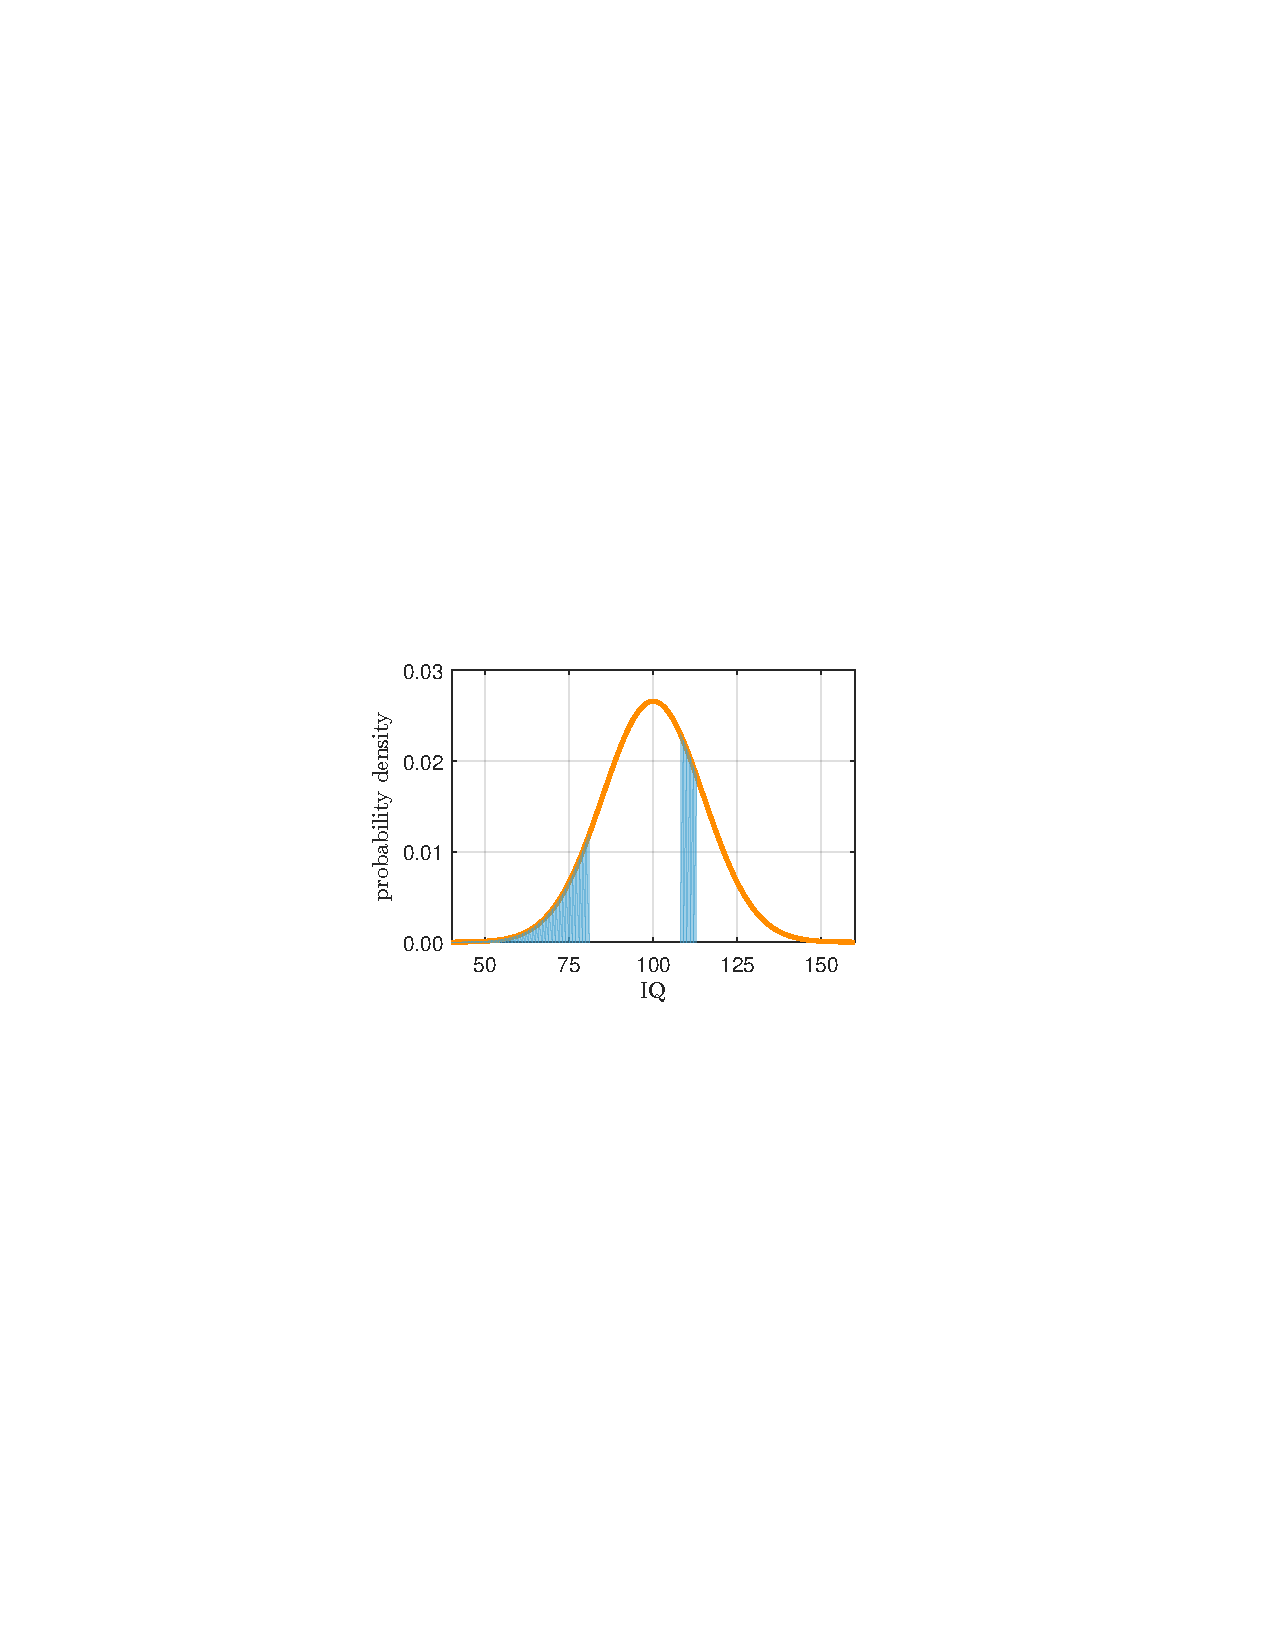
\includegraphics[scale=0.8,viewport=178 311 410 473]{figs/etzvandekerckhove_fig3.pdf}\\[1ex]
\caption{An example of a probability density function (PDF). PDFs express the relative plausibility of different values and can be used to determine the probability that a value lies in any interval. The PDF shown here is the theoretical distribution of IQ in the population: a normal distribution (a.k.a.\ Gaussian distribution) with mean 100 and standard deviation 15. In this distribution, the filled region to the left of 81 has an area of approximately 0.10, indicating that for a random member of the population, there is a 10\% chance their IQ is below 81. Similarly, the narrow shaded region on the right extends from 108 to 113 and also has an area of 0.10, meaning that a random member has a 10\% probability of falling in that region.}
\label{fig:densexample}
\end{figure}

By definition, the total area under a probability density function is 1:$$1 = \int_A p(a)da,$$ where capitalized $A$ indicates that the integration is over the entire range of possible values for the parameter that appears at the end -- in this case $a$. The range $A$ is hence a disjoint set of possible values for $a$. For instance, if $a$ is the mean of a normal distribution, $A$ indicates the range of real numbers from $-\infty$ to $\infty$; if $a$ is the rate parameter for a binomial distribution, $A$ indicates the range of real numbers between $0$ and $1$. The symbol $da$ is called the \emph{differential} and the function that appears between the integration sign and the differential is called the \emph{integrand} -- in this case $p(a)$.

We can consider how much probability is contained within smaller sets of values within the range $A$; for example, when dealing with IQ in the population, we could consider the integral over only the values of $a$ that are less than 81, which would equal the probability that $a$ is less than 81:\footnote{Strictly speaking, this integral is the probability that $a$ is less than \emph{or equal to} 81, but the probability of any single point in a continuous distribution is 0. By the sum rule, $P(a \leq 81) = P(a < 81) + P(a = 81)$, which simplifies to $P(a \leq 81) = P(a < 81) + 0$.}$$P(a < 81) = \int_{-\infty}^{81} p(a)da.$$ {In Figure~\ref{fig:densexample}, the shaded area on the left indicates the probability density over the region $(-\infty, 81)$.}

The fundamental rules of probability theory in the discrete case---the sum and product rules---have continuous analogues. The continuous form of the product rule is essentially the same as in the discrete case: $p(a,b) = p(a)p(b|a)$, where $p(a)$ is the density of the continuous parameter $a$ and $p(b|a)$ denotes the \textit{conditional density} of $b$ (i.e., the density of $b$ assuming a particular value of $a$). As in the discrete case of Equation~\ref{eq:prodrule}, it is true that $p(a,b) = p(a)p(b|a) = p(b)p(a|b)$, and that $p(a,b)=p(a)p(b)$ if we consider $a$ and $b$ to be statistically independent. For the continuous sum rule, the summation in Equation~\ref{eq:sumrule} is replaced by an integration over the entire parameter space $B$: $$p(a) = \int_B p(a,b)db.$$ Because this operation can be visualized as a function over two dimensions ($p(a,b)$ is a function that varies over $a$ and $b$ simultaneously) that is being collapsed into the one-dimensional margin ($p(a)$ varies only over $a$), this operation is alternatively called \emph{marginalization}, \emph{integrating over $b$}, or \emph{integrating out $b$}.

Using these continuous forms of the sum and product rules, we can derive a continuous form of Bayes' Rule by successively applying the continuous sum and product rules to the numerator and denominator (analogously to Equation~\ref{eq:bayesrule2}):
\begin{equation}
  \begin{array}{rcl}
    p(a|b) &=& \dfrac{p(a,b)}{p(b)} = \dfrac{p(a)p(b|a)}{p(b)}\\[3ex]
           &=& \dfrac{p(a)p(b|a)}{\int_A p(a)p(b|a)da}.
  \end{array}
  \label{eq:bayesrule3}
\end{equation}
Since the product in the numerator is divided by its own integral, the total area under the posterior distribution always equals 1; this guarantees that the posterior is always a proper distribution if the prior and likelihood are proper distributions. It should be noted that by ``continuous form of Bayes' Rule'' we mean that the prior and posterior distributions for the model parameter(s) are continuous -- the sample data can still be discrete, as in Example~{\ref{ex:vomit}} below.

One application of Bayesian methods to continuous parameters is \emph{estimation}.  If $\theta$ (theta) is a parameter of interest (say, the success probability of a participant in a task), then information about the relative plausibility of different values of $\theta$ is given by the probability density $p(\theta)$. If new information becomes available, for example in the form of new data $x$, the density can be updated and made conditional on $x$: 
\begin{equation}
  \begin{array}{rcl}
    p(\theta|x) = \dfrac{p(\theta)p(x|\theta)}{p(x)} 
                = \dfrac{p(\theta)p(x|\theta)}{\int_\Theta p(\theta)p(x|\theta)d\theta} .
  \end{array}
  \label{eq:bayesrule4}
\end{equation}

Since in the context of scientific learning these two densities typically represent our knowledge of a parameter $\theta$ before and after taking into account the new data $x$, $p(\theta)$ is often called the \emph{prior density} and $p(\theta|x)$ the \emph{posterior density}.  Obtaining the posterior density involves the evaluation of Equation~\ref{eq:bayesrule4} and requires one to define a likelihood function $p(x|\theta)$, which indicates how strongly the data $x$ are implied by every possible value of the parameter $\theta$.

The numerator on the right hand side of Equation~\ref{eq:bayesrule4}, $p(\theta)p(x|\theta)$,  is a product of the prior distribution and the likelihood function, and it completely determines the shape of the posterior distribution (note that the denominator in that equation is not a function of the parameter $\theta$; even though the parameter seems to feature in the integrand, it is in fact ``integrated out'' so that the denominator depends only on the data $x$). For this reason, many authors prefer to ignore the denominator of Equation~\ref{eq:bayesrule4} and simply write the posterior density as proportional to the numerator, as in $p(\theta|x)\propto p(\theta)p(x|\theta)$. We do not, because this conceals the critical role the denominator plays in a predictive interpretation of Bayesian inference.

The denominator $p(x)$ is the weighted-average probability {density} of the data $x$, where the form of the prior distribution determines the weights. This normalizing constant is the continuous analogue of the prior predictive distribution, often alternatively referred to as the \textit{marginal likelihood} or the Bayesian \textit{evidence}.\footnote{We particularly like Evans's take on the term Bayesian \textit{evidence}: ``For evidence, as expressed by observed data in statistical problems, is what causes beliefs to change and so we can measure evidence by measuring change in belief'' \cite[p.\ 243]{evans2014}.}  Consider that, in a similar fashion to the discrete case, we can rearrange Equation~\ref{eq:bayesrule4} as follows---dividing each side by $p(\theta)$---to illuminate in an alternative way how Bayes' rule operates in updating the prior distribution $p(\theta)$ to a posterior distribution $p(\theta|x)$:
\begin{equation}\label{eq:savdic}
  \dfrac{p(\theta|x)}{p(\theta)} = \dfrac{p(x|\theta)}{p(x)} 
                                 = \dfrac{p(x|\theta)}{\int_\Theta p(\theta)p(x|\theta)d\theta}.
\end{equation}
On the left hand side, we see the ratio of the posterior to the prior density. Effectively, this tells us for each value of $\theta$ how much more or less plausible that value became due to seeing the data $x$. The equation shows that this ratio is determined by how well that specific value of $\theta$ predicted the data, in comparison to the weighted-average predictive accuracy across all values in the range $\Theta$. In other words, \textbf{parameter values that exceed the average predictive accuracy across all values in $\Theta$ have their densities increased, while parameter values that predict worse than the average have their densities decreased} \cite<see>{moreyetalinpressprediction,WagenmakersEtAl2016benefits}. 

While the discrete form of Bayes' rule has natural applications in hypothesis testing, the continuous form more naturally lends itself to parameter estimation.  Examples of such questions are: ``What is the probability that the regression weight $\beta$ is positive?''\ and ``What is the probability that the difference between these means is between $\delta=-.3$ and $\delta=.3$?'' These questions can be addressed in a straightforward way, using only the product and sum rules of probability.

\example{Return of the Jedi's lunch}\label{ex:vomit}
In the kitchen laboratory behind \textit{Dex's Diner}, Dexter Jettster develops novelty foods for the entertainment of pilots, mechanics, and the occasional off-duty Jedi. In a recent project, Dexter is studying the effects of his infamous \emph{regurgitation rations}, which cause immediate vomiting when consumed. The target audience is Jedi younglings from the nearby Temple, who need an excuse to leave a tedious lesson and enjoy making terrible messes.

Shortly after the rations appeared beneath the diner's counter, customers began to report that regurgitation rations cause not one, but multiple ``expulsion events.'' To learn more about this unknown behavior, Dexter decides to set up an exploratory study. From scattered customer reports, he believes the expulsion rate to be between three to five events per hour, but he intends to collect data to determine the rate more precisely. At the start of this project, Dexter has no distinct hypotheses to compare -- he is interested only in estimating the expulsion rate.

Since the data $x$ are counts of the number of expulsion events within an interval of time, Dexter decides that the appropriate model for the data (i.e., likelihood function) is a Poisson distribution {(see top panel of Figure~\ref{fig:poisson})}:
\begin{equation}\label{eq:poisson}
  p(x|\rate) = \frac{1}{x!} \exp\left(-\rate\right) \rate^x,
\end{equation}
with the $\rate$ (lambda) parameter representing the expected number of events within the time interval (note $\exp(-\lambda)$ is simply a clearer way to write $e^{-\lambda}$). 

A useful prior distribution for Poisson rates is the Gamma distribution \cite[Appendix~A]{GelmanEtAl2004}:\footnote{Recall that $x!=x\times (x-1) \times \dots\times 1$ (where $x!$ is read as ``the factorial of $x$,'' or simply ``$x$ factorial''). Similarly, the Gamma function $\Gamma(\shape)$ is equal to $(\shape-1)!=(\shape-1)\times(\shape-2)\times\dots\times 1$ when $\shape$ is an integer. Unlike a factorial, however, the Gamma function is more flexible in that it can be applied to non-integers.}
\begin{equation}\label{eq:gamma}
  p(\rate|\shape,\scale) = \frac{\scale^\shape}{\Gamma(\shape)} \exp\left(-\rate \scale\right) \rate^{\shape - 1},
\end{equation}
A visual representation of the Gamma distribution is given in the second panel of Figure~\ref{fig:poisson}. A Gamma distribution has two parameters that determine its form, namely shape ($\shape$) and scale ($\scale$).\footnote{To ease readability we use Greek letters for the parameters of a likelihood function and Roman letters for the parameters of prior (posterior) distributions. The parameters that characterize a distribution can be found on the right side of the conditional bar; for instance, the likelihood function $p(x|\rate)$ has parameter $\rate$, whereas the prior distribution $p(\rate|\shape,\scale)$ has parameters $(\shape,\scale)$.} The Gamma distribution is useful here for two reasons: first, it has the right \emph{support}, meaning that it provides nonzero density for all possible values for the rate (in this case all positive real numbers); and second, it is \emph{conjugate} with the Poisson distribution, a technical property to be explained below.

Before collecting further data, Dexter makes sure to specify what he believes to be reasonable values based on the reports he has heard. In {the second panel of} Figure~\ref{fig:poisson}, he set the prior parameters to $\shape = 2$ and $\scale = 0.2$ by drawing the shape of the distribution for many parameter combinations and selecting a curve that closely resembles his prior information: Values between three and five are most likely, but the true value of the expulsion rate could conceivably be much higher.

\begin{figure}[btp]
\centering
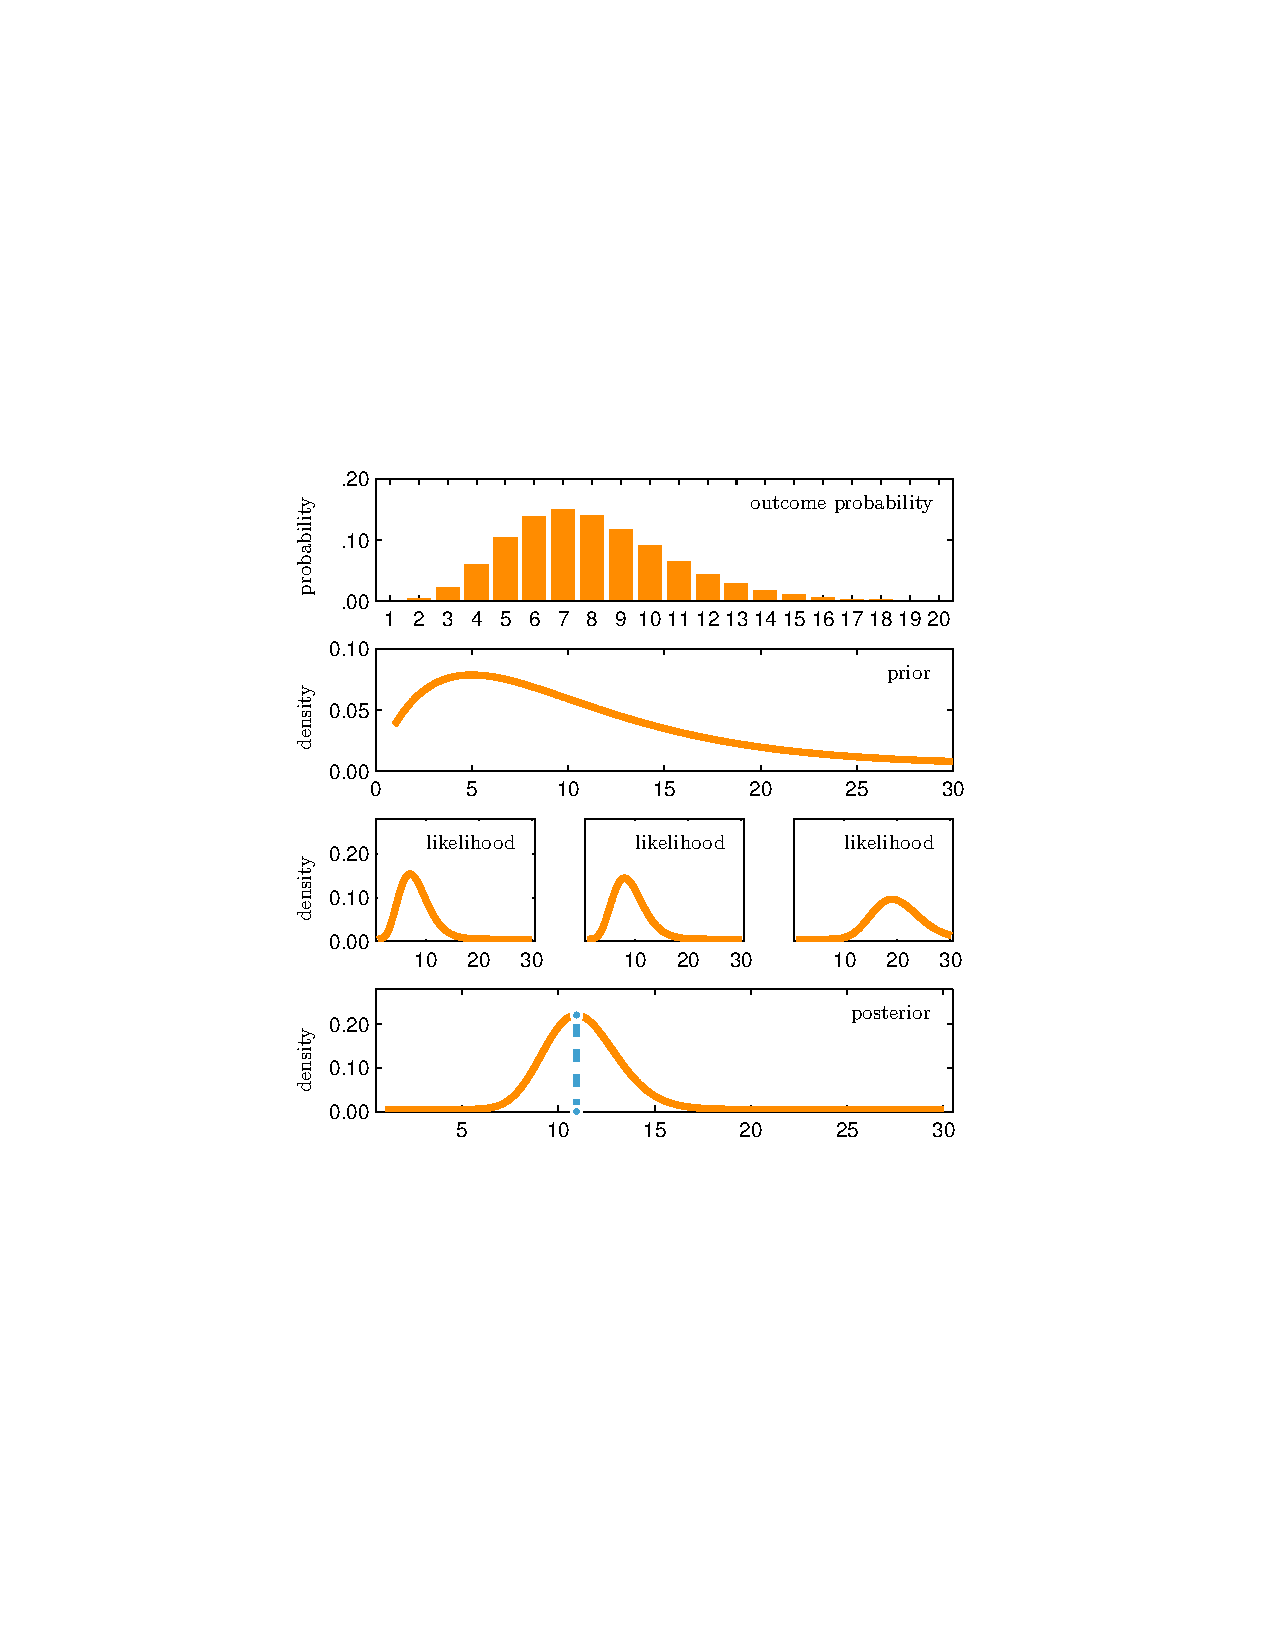
\includegraphics[width=0.5\textwidth,viewport=126 240 483 582]{figs/etzvandekerckhove_fig4.pdf}
\caption{\textbf{Top row:} An example Poisson distribution. The function is  $p(x|\lambda=7)$ as defined in Equation~\ref{eq:poisson}. The height of each bar indicates the probability of that particular outcome (e.g., number of expulsion events). \textbf{Second row:} The prior distribution of $\rate$; a Gamma distribution with parameters $\shape=2$ and $\scale=0.2$. This is the initial state of Dexter's knowledge of the expulsion rate $\rate$ (the expected number of expulsion events per hour). \textbf{Third row:} The likelihood functions associated with $x_1=7$ (left), $x_2=8$ (center), and $x_3=19$ (right). \textbf{Bottom row:} The posterior distribution of $\rate$; a Gamma distribution with parameters $\shape=36$ and $\scale=3.2$. This is the final state of knowledge regarding $\lambda$.}
\label{fig:poisson}
\end{figure}

Three volunteers are easily found, administered one regurgitation ration each, and monitored for one hour. The observed event frequencies are $x_1=7$, $x_2=8$, and $x_3=19$.

With the prior density (Equation ~\ref{eq:gamma}) and the likelihood (Equation ~\ref{eq:poisson}) known, Dexter can use Bayes' rule as in Equation~\ref{eq:bayesrule3} to derive the posterior distribution of $\lambda$, conditional on the new data points $X_n = (x_1, x_2, x_3)$. He will assume the $n=3$ data points are independent given $\lambda$, so that  their likelihoods may be multiplied.\footnote{The likelihood function of the combined data is ${p(X_n|\lambda) =p(x_1|\lambda)\times p(x_2|\lambda)\times p(x_3|\lambda)}$, which we write using the more compact product notation, $ \prod_{i=1}^{n=3}p(x_i|\lambda)$, in the following equations to save space. Similarly, $\prod_{i=1}^{n=3} \exp\left(-\rate\right) \rate^{x_i}={\exp(-3\lambda)\lambda^{(x_1+x_2+x_3)}}$.} This leaves him with the following expression for the posterior density of $(\rate|X_n,\shape,\scale)$  :\begin{eqnarray*}p(\rate|X_n,\shape,\scale) =
\frac{ \frac{\scale^\shape}{\Gamma(\shape)} \exp\left(-\rate \scale\right) \rate^{\shape - 1} \prod_{i=1}^{n=3} \frac{1}{x_i!} \exp\left(-\rate\right) \rate^{x_i} } { \int_\Lambda \frac{\scale^\shape}{\Gamma(\shape)} \exp\left(-\rate \scale\right) \rate^{\shape - 1} \prod_{i=1}^{n=3} \frac{1}{x_i!} \exp\left(-\lambda\right) \rate^{x_i} d\rate }.\end{eqnarray*}

This expression may look daunting, Dexter is not easily intimidated. He goes through the following algebraic steps to simplify the expression: (1) collect all factors that do not depend on $\rate$ (which, notably, includes the entire denominator) and call them $Q(X_n)$, and (2) combine exponents with like bases:
\begin{eqnarray*}
  p(\rate|X_n,\shape,\scale) &=& Q(X_n) \exp\left(-\rate \scale\right) \rate^{\shape - 1} 
                                 \times \prod_{i=1}^{n=3} \exp\left(-\rate\right) \rate^{x_i} \\
                             &=& Q(X_n) \exp\left[-\rate(\scale + n)\right] \rate^{\left(\shape + \sum_{i=1}^{n=3} x_i\right) - 1}.
\end{eqnarray*}

Note the most remarkable result that is obtained here! Comparing the last equation to Equation~\ref{eq:gamma}, it turns out that these have \emph{exactly the same form}.  Renaming $(\scale+n)$ to $\hat\scale$ and $\left(\shape + \sum_i^n x_i\right)$ to $\hat\shape$ makes this especially clear: $$p(\rate|X_n,\shape,\scale) = \frac{\hat\scale^{\hat\shape}}{\Gamma\left(\hat\shape\right)} \exp\left(-\rate\hat\scale\right) \rate^{\hat\shape - 1} = p(\rate|\hat\shape,\hat\scale).$$ Here, Dexter has completed the distribution by replacing the scaling constant $Q(X_n)$ with the scaling constant of the Gamma distribution -- after all, we know that the outcome must be a probability density, and each density has a unique scaling constant that ensures the total area under it is 1.

The posterior distribution $p(\rate|X_n, \shape, \scale)$ thus turns out to be equal to the prior distribution with updated parameters $\hat\scale = \scale + n$ and $\hat\shape = \shape + \sum_{i=1}^n x_i$.  Differently put, \begin{equation}p(\rate|X_n,\shape,\scale) = p\left(\rate\mid\shape + \sum_{i=1}^n x_i, \scale + n\right).\label{eq:gammapost}\end{equation} This amazing property, where the prior and posterior distributions have the same form, results from the special relationship between the Gamma distribution and the Poisson distribution: \emph{conjugacy}. The bottom panel of Figure~\ref{fig:poisson} shows the much more concentrated posterior density for $\lambda$: a Gamma distribution with parameters $\hat\shape = 36$ and $\hat\scale = 3.2$. 

When priors and likelihoods are conjugate, three main advantages follow. First, it is easy to express the posterior density because it has the same form as the prior density (as seen in Equation~\ref{eq:gammapost}). Second, it is straightforward to calculate means and other summary statistics of the posterior density. For example, the mean of a Gamma distribution has a simple formula: $\shape/\scale$. Thus, Dexter's prior density for $\rate$ has a mean of $\shape/\scale=2/.2=10$, and their posterior density for $\rate$ has a mean of $\hat\shape/\hat\scale = 36/3.2 = 11.25$. The prior and posterior densities' respective modes are $(\shape-1)/\scale=5$ and $(\hat\shape-1)/\hat\scale = 35/3.2 \approx 11$, as can be seen from Figure~\ref{fig:poisson}. Third, it is straightforward to  update the posterior distribution sequentially as more data become available.

\paragraph{Discussion}  Social scientists estimate model parameters in a wide variety of settings. Indeed, a focus on estimation is the core of the \emph{New Statistics} (\citeNP{Cumming2014}{; see also \citeNP{KruschkeSI2}}). The \emph{regurgitation ration} example illustrates how Bayesian parameter estimation is a direct consequence of the rules of probability theory, and this relationship licenses a number of interpretations that the \emph{New Statistics} does not allow. Specifically, the basis in probability theory allows Dexter to (1) point at the most plausible values for the rate of expulsion events and (2) provide an interval that contains the expulsion rate with a certain probability (e.g., a Gamma distribution calculator shows that $\lambda$ is between 8.3 and 14.5 with 90\% probability).

The applications of parameter estimation often involve exploratory settings: no theories are being tested and a distributional model of the data is assumed for descriptive convenience.  Nevertheless, parameter estimation can be used to adjudicate between theories under certain special circumstances: if a theory or hypothesis makes a particular prediction about a parameter's value or range, then estimation can take a dual role of hypothesis testing. In the social sciences most measurements have a natural reference point of zero, so this type of hypothesis will usually be in the form of a directional prediction for an effect. In our example, suppose that Dexter was specifically interested in whether $\lambda$ was less than 10.  Under his prior distribution for $\lambda$, the probability of that being the case was 59.4\%.  After seeing the data, the probability $\lambda$ is less than 10 decreased to 26.2\%.

\subsection*{Estimating the mean of a normal distribution}
By far the most common distribution used in statistical testing in social science, the normal distribution deserves discussion of its own. The normal distribution has a number of interesting properties---some of them rather unique---but we discuss it here because it is a particularly appropriate choice for modeling unconstrained, continuous data.  The mathematical form of the normal distribution is
\begin{eqnarray*}
 p(x|\mu,\sigma) &=& N(x|\mu,\sigma^2) \\
                 &=&\frac{1}{\sqrt{2\pi\sigma^2}}\exp\left[-\frac{1}{2}\left(\frac{x-\mu}{\sigma}\right)^2\right],
\end{eqnarray*}
with the $\mu$ (mu) parameter representing the average (\textit{mean}) of the population from which we are sampling and $\sigma$ (sigma) the amount of dispersion (\textit{standard deviation}) in the population. We will follow the convention that the normal distribution is parameterized with the \textit{variance} $\sigma^2$. An example normal distribution is drawn in Figure~\ref{fig:densexample}.

One property that makes the normal distribution useful is that it is \emph{self-conjugate}: The combination of a normal prior density and normal likelihood function is itself a normal distribution, which greatly simplifies the derivation of posterior densities. Using Equation~\ref{eq:bayesrule3}, and given some data set $X_n=(x_1,x_2,...,x_{n})$, we can derive the following expression for the posterior density $(\mu|X_n,a,b)$: $$p(\mu|X_n,a,b) = \dfrac{N(\mu|a,b^2)\times\prod_i^n N(x_i|\mu,\sigma^2)}{\int_{M}N(\mu|a,b^2)\times\prod_i^n N(x_i|\mu,\sigma^2)d\mu}$$ Knowing that the product of normal distributions is also a normal distribution (up to a scaling factor), it is only a matter of tedious algebra to derive the posterior distribution of $\mu$. We do not reproduce the algebraic steps here -- the detailed derivation can be found in \citeA{GelmanEtAl2004} {and \citeA{RaiffaSchlaifer1961}}, among many other places. The posterior is $$p(\mu|X_n,a,b) = N\left(\mu|\hat{a},\hat{b}^2\right),$$ where $$\hat{b}^2 = {\frac{1}{\frac{n}{\sigma^2}+\frac{1}{b^2}}}$$ and 
\begin{eqnarray*}
 \hat{a} &=& \left( \frac{\hat{b}^2}{b^2}\right)a
            +\left( \frac{\hat{b}^2}{\sigma^2/n} \right) \bar x\\[1ex]
         &=& \W a + \left(1-\W\right)\bar x,
\end{eqnarray*}
where $\bar{x}$ refers to the mean of the sample.

Carefully inspecting these equations can be instructive. To find $\hat{b}$, the standard deviation (i.e., spread) of the posterior distribution of $\mu$, we must compare the spread of the prior distribution, $b$, to the \emph{standard error of the sample}, $\sigma/\sqrt{n}$. The formula for $\hat{b}$ represents how our uncertainty about the value of $\mu$ is reduced due to the information gained in the sample. If the sample is noisy, such that the standard error of the sample is large compared to the spread of the prior, then relatively little is learned from the data compared to what we already knew before, so the difference between $\hat{b}$ and $b$ will be small. Conversely, if the data are relatively precise, such that the standard error of the sample is small when compared to the spread of the prior, then much will be learned about $\mu$ from the data and $\hat{b}$ will be much smaller than $b$. 

To find $\hat{a}$, the mean of the posterior distribution for $\mu$, we need to compute a weighted average of the prior mean and the sample mean. In the formula above, the weights attached to $a$ and $\bar x$ sum to 1 and are determined by how much each component contributes to the total precision of the posterior distribution. Naturally, the best guess for the value of $\mu$ splits the difference between what we knew of $\mu$ before seeing the sample and the estimate of $\mu$ obtained from the sample; whether the posterior mean is closer to the prior mean or the sample mean depends on a comparison of their relative precision. If the data are noisy compared to the prior (i.e., the difference between prior variance $b^2$ and posterior variance $\hat{b}^2$ is small, meaning $\W$ is near 1), then the posterior mean will stay relatively close to the prior mean. If the data are relatively precise (i.e., $\W$ is near zero), the posterior mean will move to be closer to the sample mean. If the precision of the prior and the precision of the data are approximately equal then $\W$ will be near $1/2$, so the posterior mean for $\mu$ will fall halfway between $a$ and $\bar x$. 

The above effect is often known as \textit{shrinkage} because our sample estimates are pulled back toward prior estimates (i.e., shrunk). Shrinkage is generally a desirable effect, in that it will lead to more accurate parameter estimates and empirical predictions \cite<see>{EfronMorris1977}. Since Bayesian estimates are automatically shrunk according to the relative precision of the prior and the data, incorporating prior information simultaneously improves our parameter estimates and protects us from being otherwise misled by noisy estimates in small samples.  Quoting \citeA[p.~163]{Gelman2010}: ``Bayesian inference is conservative in that it goes with what is already known, unless the new data force a change.''

Another way to interpret these weights is to think of the prior density as representing some amount of information that is available from an unspecified number of previous hypothetical observations, which are then added to the information from the real observations in the sample. For example, if after collecting 20 data points the weights come to $\W = .5$ and $1 - \W = .5$, that implies that the prior density carried 20 data points' worth of information. In studies for which obtaining a large sample is difficult, the ability to inject outside information into the problem to come to more informed conclusions can be a valuable asset. A common source of outside information is estimates of effect sizes from previous studies in the literature. As the sample becomes more precise, usually through increasing sample size, $\W$ will continually decrease, and eventually the amount of information added by the prior will become a negligible fraction of the total \cite<see also the principle of stable estimation, described in>{EdwardsEtAl1963}. 

\example{Of womp rats and offworlders}\label{ex:offworlder}
Womp rats are scavengers native to Tatooine. While typically more interested in refuse than travelers, a startled womp rat might bite a humanoid, causing a mild rash, discomfort in the affected area, and profuse sweating.

Anecdotal reports dating back to before the Empire indicate that offworlders suffer a stronger immunohistological reaction to womp-rat bites than Twi'leks. This example of physiological differences between species caught the attention of the medical droid 2-1B, who decided to investigate the issue: When bitten by a womp rat, do symptoms persist longer in the average offworlder than in the average Twi'lek?

\newcommand{\units}{hours}
\FPset{\vmw}    {42}   % Twi'lek population mean
\FPset{\vsigma} { 2}   % Twi'lek population standard deviation
\FPset{\va}     {\vmw} % Human population mean prior mean
\FPset{\vb}     { 6}   % Human population mean prior standard deviation
\FPset{\vn}     {30}   % Sample size
\FPset{\vxbar}  {43}   % Sample mean
\FPeval{\vs}    {\vsigma/(\vn^(0.5))}  % Sample standard error of estimation
\FPeval{\vbhat} {((\vn/\vsigma^2 + \vb^(-2))^(-1))^(0.5)}  % Posterior standard deviation
\FPeval{\vW}    {\vbhat^2/\vb^2}  % Updating weight W^2
\FPeval{\vahat} {\vW*\va + (1-\vW)*\vxbar}  % Posterior mean

% Mass below the reference value
\FPeval{\phitmp}{1/(1 + exp(-0.07056*((\vahat-\va)/\vbhat)^3 - 1.5976*(\vahat-\va)/\vbhat))}  % Approximation of the normal cdf...
\FPeval{\phipct}{100*\phitmp}  % The percentage of mass

% Bayes factor for the existence of a difference
\FPeval{\pdferr}{0.5*((\va-\vahat)*(\va-\vahat)/\vbhat^2)}  % \pdferr\\       % argument to exp
\FPexp{\pdfinvkernel}{\pdferr}                              % \pdfinvkernel\\ % inv normal kernel
\FPeval{\vpdfc}{0.398942280401433/(\vbhat * \pdfinvkernel)} % \vpdfc \\       % p(X|H_0)
\FPeval{\vpdfs}{0.398942280401433/\vb}                      % \vpdfs \\       % p(X|H_a)
\FPeval{\vbf}{\vb/(\vbhat * \pdfinvkernel)}                 % \vbf \\         % BF_{cs}
\FPeval{\ibf}{(\vbhat * \pdfinvkernel)/\vb}                 % \ibf \\         % BF_{sc}

The Galactic Republic medical archive keeps meticulous historical records of encounters between Twi'leks and Tatooine fauna that go back over a thousand years, so 2-1B has a great deal of information on Twi'lek reactions to womp-rat bites. Specifically, the average duration of the ensuing sweating episode is \vmw~\units, with a standard deviation of \vsigma. Due to the large amount of data available, the standard error of measurement is negligible. 2-1B's question can now be rephrased: What is the probability a womp-rat bite on an offworlder results in an average sweating episode longer than \vmw~\units?

2-1B has two parameters of interest: the population mean---episode duration $\mu$---and its corresponding population standard deviation $\sigma$. The droid has no reason to believe there is a difference in dispersion between the offworlder and Twi'lek populations, so it will assume for convenience that $\sigma$ is known and does not differ between offworlders and Twi'leks (i.e., $\sigma=2$; ideally, $\sigma$ would be estimated as well, but for ease of exposition we will take the standard deviation as known).

Before collecting any data, 2-1B must assign to $\mu$ a prior distribution that represents what it takes to be the range of plausible values for this parameter before collecting data. To characterize its background information about the population mean $\mu$, 2-1B uses a prior density represented by a normal distribution, $p(\mu|a,b)=N(\mu|a,b^2)$, where $a$ represents the location of the mean of the prior and $b$ represents its standard deviation (i.e., the amount of uncertainty we have regarding $\mu$). From its informal observations, 2-1B concludes that the mean difference between Twi'leks and offworlders will probably not be larger than \print[0]{2.5*\vb}~\units. To reflect this information, 2-1B centers the prior distribution $p(\mu|a,b)$ at $a = \vmw$~\units{} (the average among Twi'leks) with a standard deviation of $b = \vb$~\units, so that prior to running its study there is a 95\% probability $\mu$ lies between (approximately) \print[0]{\vmw-2.5758*\vb}{ }and \print[0]{\vmw+2.5758*\vb}~\units. Thus, $p(\mu|a,b) = N(\mu | \vmw, \vb^2)$.

With these prior distributions in hand, 2-1B can compute the prior probability that $\mu$ is less than $\vmw$~\units{} by finding the area under the prior distribution to the left of the benchmark value via integration. Integration from negative infinity to some constant is most conveniently calculated with the \emph{cumulative distribution function} $\Phi$:
\begin{eqnarray*}
  p(\mu < \vmw|a,b) &=& \int_{-\infty}^{\vmw}N(\mu|a,b^2)d\mu\\
                    &=& \Phi\left(\vmw | a, b^2\right),
\end{eqnarray*}
which in this case is exactly $0.5$ since the benchmark value is exactly the mean of the prior density: 2-1B centered its prior on \vmw{ }and specified that the offworlder sweating duration could be longer or shorter with equal probability.

2-1B collects information on a representative sample of \vn{ }offworlder volunteers treated for womp-rat bites at a Rebel field hospital. It finds a sample mean of $\bar x = \vxbar$ and standard error of $s = \sigma/\sqrt{n} = \vsigma/\sqrt{\vn} = \print{\vs}$. 2-1B can now use the data and the above formulas to update what it knows about $\mu$.

Since the spread of the prior for $\mu$ is large compared to the standard error of the sample ($b = \vb$ versus $s = \print{\vs}$), 2-1B has learned much from the data and its posterior density for $\mu$ is much less diffuse than its prior: $$\hat{b} = \sqrt{\frac{1}{\frac{1}{s^2}+\frac{1}{b^2}}} = \sqrt{\frac{1}{\frac{1}{\print{\vs}^2}+\frac{1}{\vb^2}}} = \print{\vbhat}.$$ With $\hat{b}$ in hand, 2-1B can find the weights needed to average $a$ and $\bar x$: $\W = (\print{\vbhat}/\vb)^2 = \print{\vW}$ and $1-\W = \print{1-\vW}$, thus $\hat{a} = \print{\vW} \times \va + \print{1-\vW} \times \vxbar = \print{\vahat}$~\units.  In summary, 2-1B's prior distribution for $\mu$, $p(\mu|a,b) = N(\mu|\va,\vb^2)$, is updated into a much more informative posterior distribution, $p(\mu|\hat{a},\hat{b}) = N(\mu | \print{\vahat}, \print{\vbhat}^2)$. This posterior distribution is shown in the left panel of Figure~\ref{fig:offworlder}; note that the prior density looks nearly flat when compared to the much more peaked posterior density.

Now that the posterior distribution of $\mu$ is known, 2-1B can revisit the original question: What is the probability that $\mu$ is greater than \va~\units? The answer is again obtained by finding the area under the posterior distribution to the right of the benchmark value via integration:
\begin{eqnarray*}
  p(\mu > \va | \hat{a}, \hat{b})
	&=& \int_{\va}^{\infty}N(\mu | \hat{a},\hat{b}^2)d\mu \\
	&=& 1 - \int_{-\infty}^{\va}N(\mu | \hat{a},\hat{b}^2)d\mu \\
    &=& 1 - \Phi\left(\va | \hat{a},\hat{b}^2\right) \\
    &=& 1 - \Phi\left(\va | \print{\vahat},\print{\vbhat}^2\right) \approx \print[4]{\phitmp}.
\end{eqnarray*}

In summary, the probability that the reaction to womp-rat bites in the average offworlder is greater than in the average Twi'lek increases from exactly $50\%$ to $\print[2]{\phipct}\%$.

\paragraph{Discussion} The conclusion of a Bayesian estimation problem is the full posterior density for the parameter{(s)}. That is, once the posterior density is obtained then the estimation problem is complete. However, researchers often choose to report summaries of the posterior distribution that represent its content in a meaningful way. One common summary of the posterior density is a \emph{posterior (credible) interval}. Credible intervals have a unique property: as \citeA{EdwardsEtAl1963} put it, ``The Bayesian theory of interval estimation is simple. To name an interval that you feel 95\% certain includes the true value of some parameter, simply inspect your posterior distribution of that parameter; any pair of points between which 95\% of your posterior density lies defines such an interval'' (p.~213). This property is made possible by the inclusion of a prior density in the statistical model \cite{Rouder2016freelunch}. It is important not to confuse credible intervals with \emph{confidence intervals}, which have no such property in general \cite{MoreyEtAlinpressCI}. Thus, when 2-1B reports that there is a \print[2]{\phipct}\% probability that $\mu$ lies between \va{ }and positive infinity~\units, it is reporting a \print[2]{\phipct}\% credible interval. It is important to note that there is no unique interval for summarizing the posterior distribution; the choice depends on the context of the research question.

\section*{Model comparison}
\epigraph{[M]ore attention [should] be paid to the precise statement of the alternatives involved in the questions asked. It is sometimes considered a paradox that the answer depends not only on the observations but on the question; it should be a platitude.}{H.~\citeA{Jeffreys1939}}

\noindent Consider the following theoretical questions. Is participant performance different than chance? Does this gene affect IQ? Does stimulus orientation influence response latency? For each of these questions the researcher has a special interest in a particular parameter value and entertains it as a possibility. However, when we estimate a parameter using a continuous distribution the answers to each of these questions is necessarily ``yes.'' To see why, recall that a probability density function specifies how much probability exists \emph{near}---not \emph{at}---a particular value of the parameter. That is, with a continuous probability distribution, probability only exists within a given \textit{range} of the parameter space; the probability of any \textit{single point} within the distribution is zero. This is inconsistent with our belief that a specified parameter value might hold true. Moreover, this poses a problem for any research question that focuses on a single value of a continuous parameter, because if its prior probability is zero then no amount of data can cause its posterior probability to become anything other than zero.

A simple but brilliant solution to this problem was first executed by \citeA{Haldane1932} but is credited mostly to \citeauthor{Jeffreys1939} (1939; see \citeNP{EtzOrigin}).  The solution involves applying the sum and product rules \emph{across multiple independent statistical models at once}. We can specify multiple separate models that have different implications about the parameter of interest, call it $\theta$, and calculate the probability of each model after data are collected. One model, say $\H_0$, says $\theta$ is equal to a single special value denoted $\theta_0$. A second model, say $\H_1$, says $\theta$ is unknown and assigns it a continuous prior density, implying $\theta$ is not equal to $\theta_0$. After collecting data $X$, there are two main questions to answer: (1) What is $P(\H_0|X)$, the posterior probability that $\theta=\theta_0$? And (2) what is  $p(\theta|X,\H_1)$, the posterior distribution\footnote{Note that we will now be using probabilities and probability densities side-by-side. In general, if the event to which the measure applies (i.e., what is to the left of the vertical bar) has a finite number of possible values, we will consider probabilities and use uppercase $P(\cdot)$ to indicate that. If the event has an infinite number of possible values in a continuum, we will consider probability densities and use lowercase $p(\cdot)$. In the case of a joint event in which at least one component has an infinite set of possibilities, the joint event will also have an infinite set of possibilities and we will use probability densities there also.}
of $\theta$ under $\H_1$ (i.e., considering the new data $X$, if $\theta\neq\theta_0$ then what might $\theta$ be)?

As before, this scenario can be approached with the product and sum rules of probability. The setup of the problem is captured by Figure~\ref{fig:hier} (focusing for now on the left half). We start at the initial fork with two potential models: $\H_0$ and $\H_1$. This layer of analysis is called the \textit{model space}, since it deals with the probability of the models. Subsequently, each model implies some belief about the value of $\theta$. This layer of analysis is called the \textit{parameter space} since it specifies what is known about the parameters within a model, and {it is important to note that} each model has its own independent parameter space. Under $\H_0$ the value of $\theta$ is known to be equal to $\theta_0$, so all of its probability is packed into a ``spike'' (a \emph{point mass}) at precisely $\theta_0$. Under $\H_1$ the value of $\theta$ is unknown and we place a probability distribution over the potential values of $\theta$ in the form of a \emph{conditional prior density}. Each model also makes predictions about what data will occur in the experiment {(i.e., the model's prior predictive distribution)}, information represented by each model's respective \textit{sample space.} We then condition on the data we observe, which allows us to update each layer of the analysis to account for the information gained. Below is a step-by-step account of how this is done{, but we remind readers that they should feel free to skip this technical exposition and jump right into the next examples.}

We answer our questions in reverse order, first deriving the posterior distribution of $\theta$ under $\H_1$, for a reason that will become clear in a moment. In this setup there are events that vary among three dimensions: $X$, $\theta$, and $\H_1$. When joint events have more than two components, the product rule decomposes $p(X,\theta,\H_1)$ one component at a time to create a chain of conditional probabilities and densities (for this reason the product rule is also known as the \textit{chain rule}). This was seen above in Example~\ref{ex:assign}. These chains can be thought of as moving from one layer of Figure~\ref{fig:hier} to the next. Thus, since we could choose any one of the three events to be factored out first, the product rule creates three possible initial chains with two probabilities per chain,
\begin{eqnarray*}
  p(X,\theta,\H_1) & = & P(\H_1)p(X,\theta|\H_1)   \\
                   & = & P(X)p(\theta,\H_1|X)      \\
                   & = & p(\theta)p(X,\H_1|\theta).
\end{eqnarray*}
(where the use of $P(X)$ or $p(X)$ depends on whether the data are discrete or continuous; we assume they are discrete here).

A natural choice is to work with the first formulation, $p(X,\theta,\H_1)=P(\H_1)p(X,\theta|\H_1)$, since $P(\H_1)$, the prior probability of the model, is known to us (it corresponds to the probability we take the right fork at the start of Figure~\ref{fig:hier}). The product rule can then be applied again to the remaining joint probability on the right hand side as follows: 
\begin{equation}\label{eq:rhs1}
  P(\H_1) \times p(X,\theta|\H_1) = P(\H_1) \times P(X|\H_1)p(\theta|X,\H_1),
\end{equation}
By symmetry of the product rule, we can also write 
\begin{equation}\label{eq:rhs2}
  P(\H_1) \times P(X,\theta|\H_1) = P(\H_1) \times p(\theta|\H_1)P(X|\theta,\H_1).
\end{equation}
If we now equate the right hand sides of Equations~\ref{eq:rhs1} and~\ref{eq:rhs2}, we can divide out $P(\H_1)$ and $P(X|\H_1)$:
\begin{eqnarray*}
  P(\H_1)P(X|\H_1)p(\theta|X,\H_1) &=& P(\H_1)p(\theta|\H_1)P(X|\theta,\H_1)\\[1ex]
  p(\theta|X,\H_1) &=& \frac{p(\theta|\H_1)P(X|\theta,\H_1)}{P(X|\H_1)}
\end{eqnarray*}
and by recognizing that ${P(X|\H_1)=\int_\Theta p(\theta|\H_1)P(X|\H_1,\theta)d\theta}$ by way of the sum rule, we are left with the following:
\begin{equation}\label{eq:MCpost}
  p(\theta|X,\H_1) = \dfrac{p(\theta|\H_1)P(X|\theta,\H_1)}{\int_\Theta p(\theta|\H_1)P(X|\theta,\H_1)d\theta}.
\end{equation}
This last formula is identical to the continuous form of Bayes' Rule (Equation~\ref{eq:bayesrule3}), where now each term is also conditional on $\H_1$.

The implication of this finding is that it is possible to perform inference using the distribution of $\theta$ under $\H_1$, $p(\theta|X,\H_1)$, \emph{ignoring everything relating to other models}, since no other models (such as $\H_0$) feature in this calculation. As before, the denominator is known as the \textit{marginal likelihood} for $\H_1$, and represents a predictive distribution for potential future data, $P(X|\H_1)$. This predictive distribution is shown in the sample space under $\H_1$ in Figure~\ref{fig:hier}, and can be thought of as the average prediction made across all possible parameter values in the model (weighted by the conditional prior density). Once the data are collected and the result is known, we can condition on the outcome and use it to update $p(\theta|\H_1)$ to obtain $p(\theta|X,\H_1)$. 

To answer our first question---what is $P(\H_0|X)$?---we need to find our way back to the discrete form of Bayes' Rule (Equation~\ref{eq:bayesrule2}). Recall that for hypothesis testing the key terms to find are $P(X|\H_0)$ and $P(X|\H_1)$, which can be interpreted as how accurately each hypothesis predicts the observed data in relation to the other. Since the parameter space under $\H_0$ is simply $\theta=\theta_0$, we can write $P(X|\H_0) = P(X|\theta_0)$. However, since the parameter space under $\H_1$ includes a continuous distribution, we need to find $\H_1$'s average predictive success across the whole parameter space, $P(X|\H_1)=\int_\Theta p(\theta|\H_1)P(X|\H_1,\theta)d\theta$. Conveniently, as we just saw above in Equation~\ref{eq:MCpost}, this is also the normalizing constant in the denominator of the posterior distribution of $\theta$ under $\H_1$. Hence, the discrete form of Bayes' Rule for hypothesis testing can be rewritten as
\begin{multline*}
  P(\H_1|X) = \dfrac{P(\H_1) P(X|\H_1)}{P(\H_1)P(X|\H_1)+P(\H_0)P(X|\H_0)}\\[3ex]
            = \dfrac{P(\H_1) \int_\Theta p(\theta|\H_1)P(X|\theta,\H_1)d\theta}{P(\H_1)
                \int_\Theta p(\theta|\H_1)P(X|\theta,\H_1)d\theta+P(\H_0)P(X|\theta_0)}.
\end{multline*}
Furthermore, in cases of model comparison between a ``point null'' (i.e., an hypothesis that, like our $\H_0$, involves a prior point mass on some parameter) and an alternative with a continuous prior for the parameter, one can rewrite the odds form of Bayes' Rule from Equation~\ref{eq:bayesodds} as follows:
$$\begin{array}{rcl}
  \underbrace{\dfrac{P(\H_1|X)} {P(\H_0|X)}}_\text{Posterior odds} &=&
  \dfrac{P(\H_1)}{P(\H_0)} \ \times \
  \dfrac{P(X|\H_1)}{P(X|\H_0)}\\[3ex]
  &=&
  \underbrace{\frac{P(\H_1)}{P(\H_0)}}_\text{Prior odds} \ \times \
  \underbrace{\frac{\int_\Theta p(\theta|\H_1)P(X|\theta,\H_1)d\theta}{P(X|\theta_0)}}_{\text{Bayes factor} ~(BF_{10})},
\end{array}$$ where the Bayes factor is the ratio of the marginal likelihoods from the two models, and its subscript indicates which models are being compared ($BF_{10}$ means $\H_1$ is in the numerator versus $\H_0$ in the denominator).

Finally, we point out one specific application of Bayes' rule that occurs when certain values of $\theta$ have a special theoretical status. For example, if $\theta$ represents the difference between two conditions in an experiment, then the case $\theta=0$ will often be of special interest (see also \citeNP{RouderSI}). Dividing each side of Equation~\ref{eq:MCpost} by $p(\theta|\H_1)$ allows one to quantify the change in the density at this point: $$\frac{p(\theta=0|X,\H_1)}{p(\theta=0|\H_1)} = \frac{P(X|\theta=0,\H_1)}{\int_\Theta p(\theta|\H_1)p(X|\theta,\H_1)d\theta} = BF_{01}.$$ This change in density is known as the Savage--Dickey density ratio or the Savage--Dickey representation of the Bayes factor (\citeNP{Dickey1971}; see also \citeNP{WagenmakersEtAl2010SDPsychologists}, and \citeNP{WagenmakersSI}; and see also \citeNP{marin2010resolving}, for some cautionary notes). When it applies, the Savage--Dickey ratio allows for an especially intuitive interpretation of the Bayes factor: If the point null value is lower on the alternative model's conditional posterior density than its prior density, the Bayes factor supports $\H_1$ over $\H_0$ by the ratio of their respective heights, and vice-versa.

The conditions under which the Savage--Dickey ratio applies are typically met in practice, since they correspond to the natural way one would build nested models for comparison {(for a good discussion on the different types of nested models see \citeNP{ConsonniVeronese2008}, Section 2)}. Namely, that all facets of the models are the same except that the smaller model fixes $\theta$ to be $\theta_0$. In our development above there is only one parameter so this condition is automatically satisfied. If, however, we have additional parameters common to both models, say $\phi$, then the Savage-Dickey ratio is obtained using the marginal prior and posterior densities, $p(\theta=\theta_0|X,\H_1)/p(\theta=\theta_0|\H_1)$, where the marginal distribution is found using the sum rule, $p(\theta|X,\H_1)=\int_\Phi p(\phi,\theta|X,\H_1)d\phi$. For this to be a proper representation of the Bayes factor, we must ensure that the conditional prior for $\phi$ under $\H_1$, when $\theta=\theta_0$, equals the prior density for $\phi$ under $\H_0$. In other terms, the Savage-Dickey representation holds only if the parameters are statistically independent a priori: $p(\phi|\theta=\theta_0,\H_1) = p(\phi|\H_0)$.

Above, our motivation for model comparison was that we wanted to test the hypothesis that a parameter took a single specified value. However, model comparison is not limited to cases where point nulls are tested. The above formulation allows us to compare any number of different types of models by finding the appropriate $P(X|\H)$. Models do not need to be nested or even have similar functional forms; in fact, the models need not be related in any other way than that they make quantitative predictions about the data that have been observed. For example, a non-nested comparison might pit a model with a mostly positive prior distribution for $\theta$ against a model where the support of the prior distribution for $\theta$ is restricted to negative values only. Or rather than a precise point null we can easily adapt the null model such that we instead compare $\H_1$ against model $\H_S$, which says $\theta$ is ``small.''  Extending model comparison to the scenario where there are more than two (but finitely many) competing models $\H_k$ is similar to before, in that
\begin{eqnarray}\label{eq:modsel}
  P(\H_i|X) =\frac{P(\H_i) p(X|\H_i)}{\sum_k P(\H_k)p(X|\H_k)}.
\end{eqnarray}

In practice, Bayes factors can be difficult to compute for more complicated models because one must integrate over possibly very many parameters to obtain the marginal likelihood \cite{KassRaftery1995,Wasserman2000}. Recent computational developments have made the computation of Bayes factors more tractable, especially for common scenarios \cite{LoveSI,WagenmakersSI}. For uncommon or complex scenarios, one might resort to reporting a different model comparison metric that does not rely on the marginal likelihood, such as the various information criteria (AIC, BIC, DIC, WAIC) or leave-one-out cross validation \cite<LOOCV; see>{SpiegelhalterEtAl2002,VandekerckhoveEtAl2015MPT,VehtariOjanen2012}. {However, it should be emphasized that for the purposes of inference these alternative methods can be suboptimal.}

\example{The Muun correction}
Proud of its work on womp-rat bite sensitivity, 2-1B (from Example~\ref{ex:offworlder}) decides to present the results at a xenomedicine symposium held in the upper levels of Coruscant. As required by Republic Archive transparency statutes, the droid has made all its data and methods publicly available ahead of time and is confident that the findings will withstand the review of the audience at this annual meeting. It delivers a flawless presentation that culminates in the conclusion that offworlders are, indeed, slightly more sensitive to womp-rat bites than Twi'leks are. The evidence, it claims, is right there in the data.

After the presentation, 2-1B is approached by San Hill---a modestly endowed Muun aristocrat---with a simple comment on the work: ``Doctor, you have not told us the evidence for your claim.''

``In fact,'' continues Hill, ``given your prior distributions for the difference between offworlders and Twi'leks, you have not even \emph{considered} the possibility that the true difference might be exactly zero, and your results merely noise. In other words, you are putting the repulsorcart before the bantha because you estimate a population difference before establishing that {evidence for} one exists. If I have reservations about whether the sarlacc even exists, it does not help for you to estimate for me the width of the creature's maw! Instead, let us ascertain how much more stock we should put in \textit{your} claim over the \textit{more parsimonious} claim of no difference between the respective population means.''

2-1B is unfazed by the aristocrat's challenge and projects the following equations as blue holograms in the air between them:
$$\begin{array}{rll}
  \H_s: & \mu \sim N(\va, \vb) & \\
  \H_c: & \mu   =  \va         & 
\end{array}$$
``These,'' 2-1B says, ``are our respective hypotheses. I claim that offworlders have different symptom durations on average than Twi'leks. I have prior information that completes my model. Your claim is that the population means may be exactly equal. In order to quantify the relative support for each of these hypotheses, we need a Bayes factor. Luckily, in this case the Bayes factor is quite easy to calculate with the Savage-Dickey density ratio, like so\dots
\begin{eqnarray*}
\frac{p(\mu| X, \H_s)}{p(\mu|\H_s)}
   &=& \frac{p(\mu| X,\H_s)}{p(\mu|\H_s)} \\
   &=& \frac{N(\mu| \hat{a}, \hat{b}^2)}{N(\mu|a,b^2)}
\end{eqnarray*}
``Now that we have derived the ratio of posterior to prior density, all that remains is to plug in the values of the parameters and to compute the ratio of Gaussian densities at the specified points\dots''

\begin{align*}
  BF_{cs} &=  \frac{N(\va \,|\, \print{\vahat}, \print{\vbhat}^2)}{N(\va \,|\, \va, \vb^2)}\\
          &=  \frac{\print{\vpdfc}}{\print{\vpdfs}} = \print{\vbf} = \frac{1}{\print{\ibf}}
\end{align*}

``A Bayes factor of not even three favors your hypothesis. You have essentially \textit{no} evidence for your claim,'' says Hill, before turning on a narrow heel and leaving 2-1B alone in the conference room.

\begin{figure}[bt]
\centering
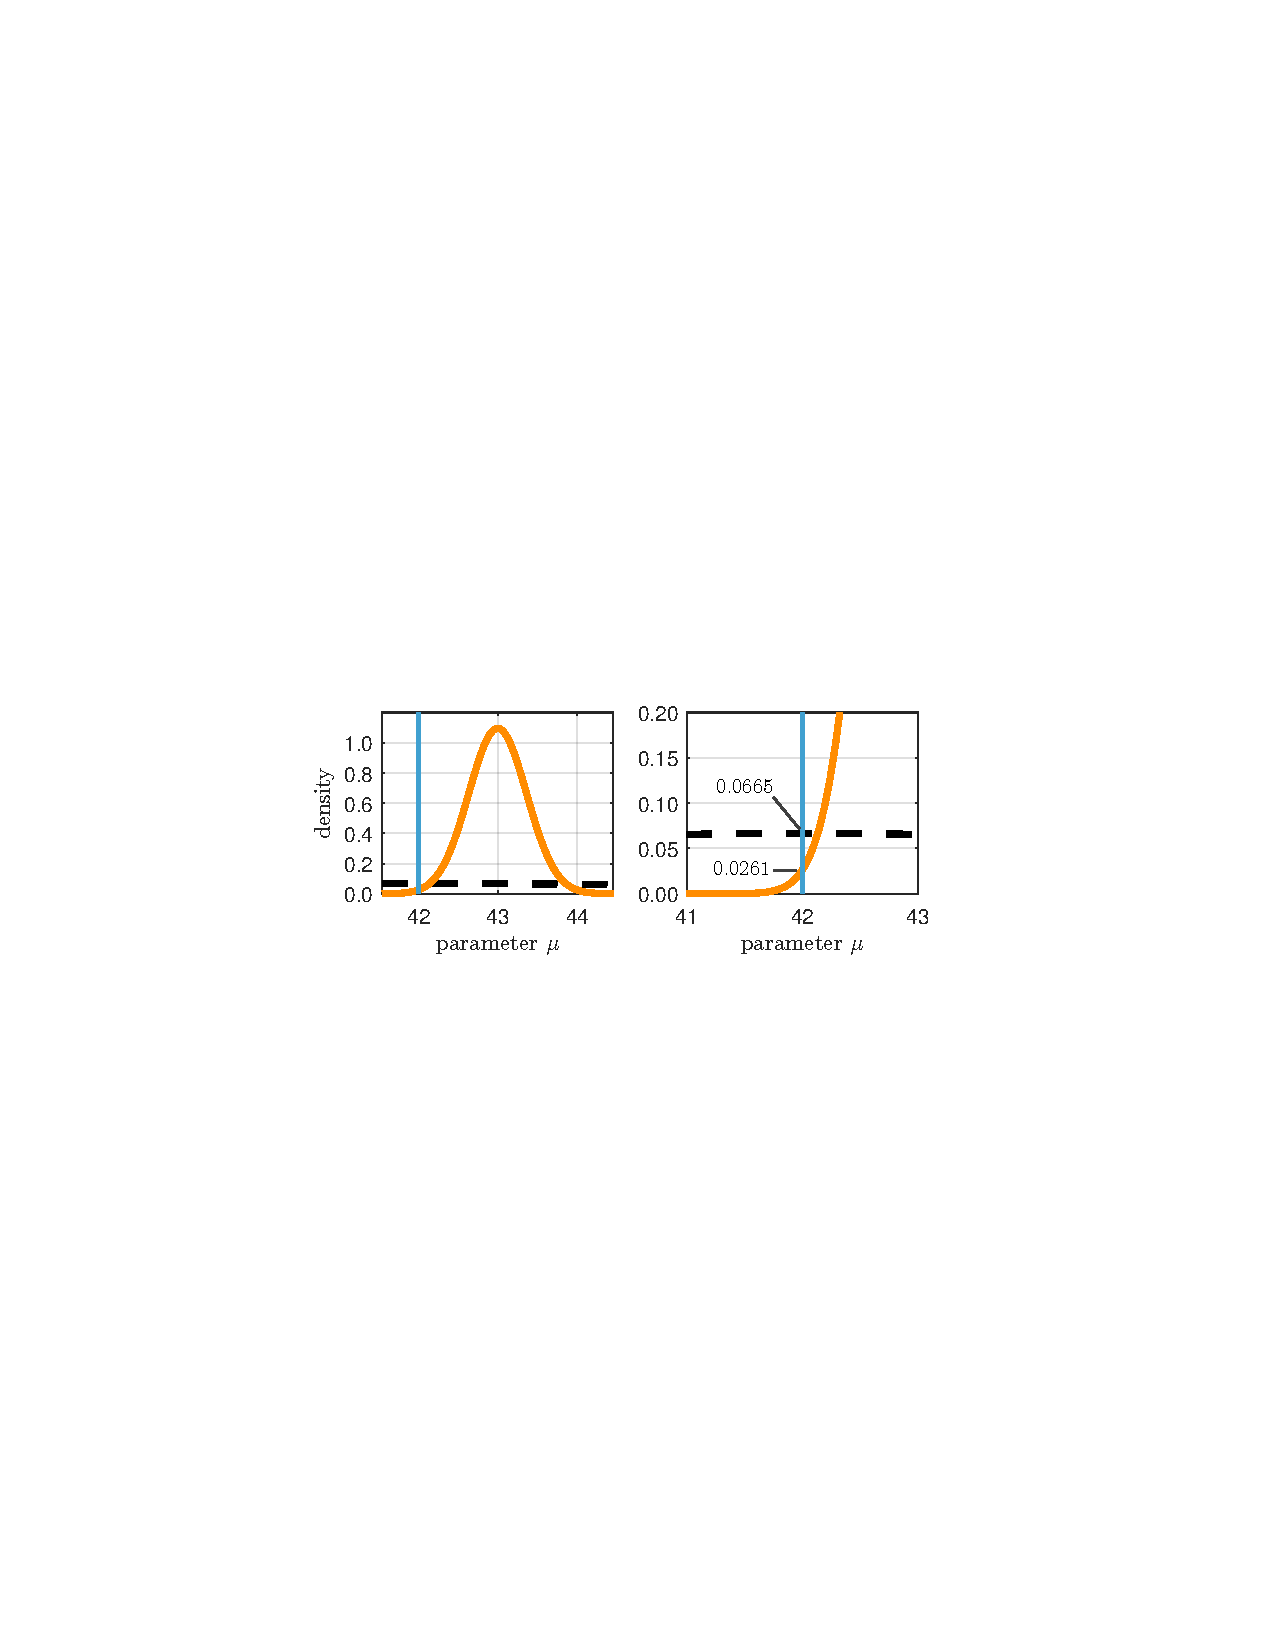
\includegraphics[width=0.5\textwidth,viewport=150 333 445 453]{figs/etzvandekerckhove_fig5.pdf}\vspace{2ex}
\caption{A closer look at the prior (dashed) and posterior (solid) densities involved in 2-1B's study on the relative sensitivity of Twi'leks and offworlders to womp-rat bites. The left panel shows the location of the fixed value (\vmw) in the body of the prior and posterior distributions. The right panel is zoomed in on the density in the area around the fixed value. Comparing the prior density to the posterior density at the fixed value reveals that very little was learned about this specific value: the density under the posterior is close to the density under the prior and amounts to a Bayes factor of approximately 3 supporting a deviation from the fixed value.}\label{fig:offworlder}
\end{figure}

\paragraph{Discussion} What has happened here? At first glance, it appears that 2-1B had strong evidence that offworlders are more sensitive than Twi'leks to womp-rat bites, and now the evidence appears to have vanished. To resolve the paradox, it is important to appreciate a few facts. First, in Example~\ref{ex:offworlder}, 2-1B indeed did not consider the hypothesis $\H_c$ that $\mu = \vmw$. In fact, because a continuous prior density was assigned to $\mu$, the prior probability of it taking on any particular value is zero.

The paradox occurs in part because of a confusion between the hypotheses being considered. While in our example, San Hill wishes to compare an ``existence'' and a ``nonexistence'' hypothesis, 2-1B started out from an existence assumption and arrives at conclusions about \emph{directionality} \cite<see also>{marsman2016}.

Implicitly, there are four different models being considered in all. There is $\H_c$, which specifies no effect, and $\H_s$, which specifies \emph{some} effect, but also $\H_-$, which specifies an effect in the negative direction, and $\H_+$, which specifies an effect in the positive direction. These last two models are concealed by 2-1B's original analysis, but its model specification implies a certain probability for the events $(\mu < \vmw)$ and $(\mu > \vmw)$. Indeed, because we know that the probability that offworlders are more (vs.~less) sensitive than their Twi'lek counterparts increased from $P(\mu > \vmw) = 50\%$ to $P(\mu > \vmw|X) = \print[2]{\phipct}\%$, we can compute Bayes factors for this case as well. In odds notation, the prior odds were increased from 1 to \FPeval{\tmp}{round(\phipct/(100-\phipct),0)}\tmp;  the Bayes factor, found by taking the ratio of posterior to prior odds, is in this case equal to the posterior odds. 2-1B's test for direction returns a much stronger result than San Hill's test of existence.

As a rule, inference must be limited to the hypotheses under consideration: No method of inference can make claims about theories not considered or ruled out a priori. Moreover, the answer we get naturally depends on the question we ask. The example that follows involves a very similar situation, but the risk of the paradox is avoided by making explicit all hypotheses under consideration.

\example{The measure of a droid} \label{ex:droid}
In the waning days of the Galactic Senate, Imperial law distinguishes between two classes of intelligent inhabitants. \emph{Citizens}, such as humans, Twi'leks, and Mon Calamari, may own property and petition the courts. By contrast, \emph{Property} includes machines that are presumed incapable of independent judgment. Recently, the classification of droids has become a matter of contention. On one side of the debate is Grand Moff Tarkin, who claims that droids are so far beneath organic intelligence that they should remain Property; on the other side is Senator Bail Organa, who argues that droids are as intelligent as organics and should be Citizens, with all the rights and responsibilities thereof.\newcommand{\cogs}{{C.O.G.S.\xspace}} The Senate convenes the \emph{Committee on Organic and General-machine Sentience} (\cogs), an ad-hoc expert committee. \cogs{} in turn calls on analysis droid K2SO to decide whether droids are indeed as intelligent as organics.

K2SO knows he will be asked to testify before \cogs{} and takes note of the composition of the three-member committee. The committee's chairperson is Mon Mothma, a venerable and wise senator who is known for her impartiality and for being of open mind to all eventualities. However, the junior members of \cogs{} are not so impartial: one member is Tarkin, the organic supremacist who believes that organics are more intelligent than droids; the other is Bail Organa, a strong egalitarian who believes that droids are equal in intelligence to organics.

K2SO begins his task by formalizing three basic hypotheses. He will call the population's average wide-spectrum intelligence quotient (WIQ) $\mu_w$ for organic wetware and $\mu_e$ for electronic droids. He can now call the difference between the population means $\delta = \mu_w - \mu_e$ so that $\delta$ captures how much \emph{more} intelligent organics are. If organics and droids are equally intelligent, $\delta=0$. If they are not, $\delta$ can take on nonzero values. We can restate this as an hypothesis of approximately no difference ($\H_0$), an hypothesis of substantial positive difference ($\H_+$; organics much more intelligent than droids), and an hypothesis of substantial negative difference ($\H_-$; droids much more intelligent than organics):
\begin{eqnarray*}
  \H_0: & \delta \approx 0\\
  \H_+: & \delta >       0\\
  \H_-: & \delta <       0.
\end{eqnarray*}
However, it is not enough to state simply that $\delta < 0$ because as a model for data, it is underspecified: no quantitative predictions follow (i.e., the likelihood for a specific data set cannot be calculated). In order to be more specific, K2SO consults with \cogs{} and together they decide on three concrete models:\footnote{$I(\cdot)$ is the \emph{indicator function}, which takes the value $1$ if its argument is true and $0$ otherwise; here it takes the role of a truncation. Since these distributions are truncated, they must be multiplied by a suitable constant such that they integrate to 1 (i.e., we \textit{renormalize} them to be proper distributions).}
\begin{center}\begin{tabular}{rrll}
  $p(\delta|\H_0)$ &=& $I(-5 < \delta < 5)/10$         & { if }$-5 < \delta < 5$\\
  $p(\delta|\H_+)$ &=& $2N(\delta|5,15)I(\delta>5)$    & { if }$\delta > 5$\\
  $p(\delta|\H_-)$ &=& $2N(\delta|-5,15)I(\delta< -5)$ & { if }$\delta < -5$.
\end{tabular}\end{center}
$\H_0$ is the assumption that the true difference $\delta$ is somewhere between $-5$ and $5$ with all values equally likely -- a uniform distribution. This is based on a consensus among \cogs{} that differences of only five WIQ points are negligible for the Senate's classification purposes: differences in this range are \emph{practically equivalent to zero}. Under $\H_+$, it is assumed that organics score at least 5 points higher than droids on average ($\delta > 5$) but differences of 20 are not unexpected and differences of 40 possible, if unlikely. Under $\H_-$, it is assumed that organics score at least 5 points \emph{lower} than droids ($\delta < -5$).

\begin{figure*}[bth]
\centering
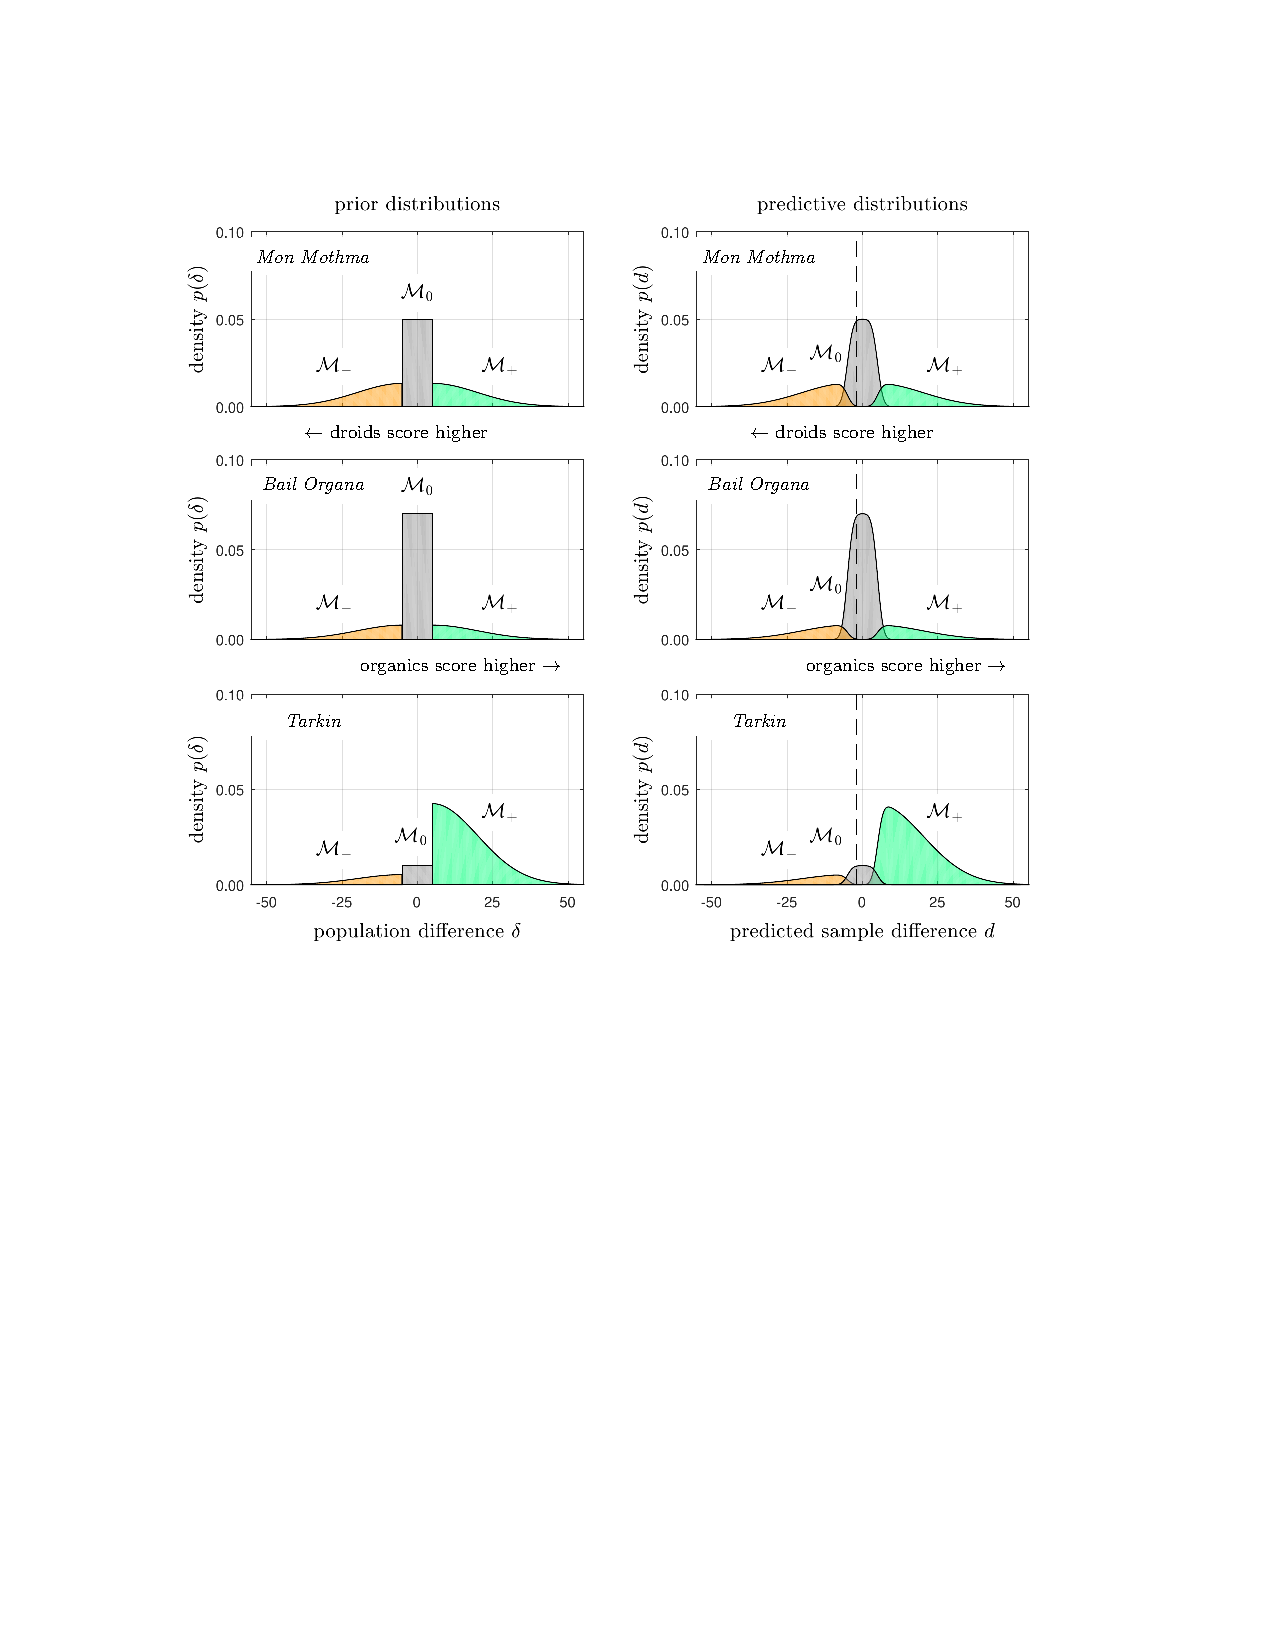
\includegraphics[scale=1.05,viewport=90 340 494 698]{figs/starwars_fig6}\vspace{2ex}
\caption{\textbf{Left:} Each of the three panel members has their own prior probability on each of the three possible models $\H_-$, $\H_0$, and $\H_+$. In this scenario, the three models do not overlap in the parameter space: no parameter value is supported by more than one model. However, this is merely a convenient feature of this example and not a requirement of Bayesian model selection -- it is entirely possible (and common) for two different models to support the same parameter value. \textbf{Right:} The predicted observed difference in a sample with a standard error of estimation of 1.5. Here, the predictive distribution for each model has been multiplied by the prior probability for that model. This representation has the interesting property that the posterior ratio between two models, given some observed difference, can be read from the figure as the ratio between the heights of the two corresponding densities. Note, for example, that at the dashed vertical line (where $d=2$), the posterior probability for $\H_0$ is higher than that for $\H_-$ or $\H_+$ for every judge.  If the distributions had not been scaled by the prior probability, these height ratios would give the Bayes factor.}
\label{fig:elffig}
\end{figure*}

After having determined the three hypotheses that \cogs{} wishes to consider, K2SO decides to collect one more piece of information: how strongly each member of the committee believes in each of the three options. He provides each member with 100 tokens and three cups, and gives them the following instructions: \begin{quote} I would like you to distribute these 100 tokens over these three cups. The first cup represents $\H_-$, the second $\H_0$, and the third $\H_+$. You should distribute them proportionally to how strongly you believe in each hypothesis.\end{quote} Mon Mothma's inferred prior probabilities of each of the three hypotheses are $(25,50,25)$, Bail Organa's are $(15,70,15)$, and Tarkin's are $(5,15,80)$. {This type of procedure is known as \textit{prior elicitation}; for more in-depth discussion on prior elicitation, see \citeA{Garthwaite2005} and \citeA{LeeSI}.}

To summarize the different prior expectations, K2SO constructs a figure to display the marginal distribution of the effect size $\delta$ for each committee member. This marginal prior density is easily obtained with the sum rule: \begin{eqnarray*} p(\delta) &=& \sum_{h \in \left(\H_-,\H_0,\H_+\right)}p(h)p(\delta|h) \\ &=& p(\H_-)p(\delta|\H_-) + p(\H_0)p(\delta|\H_0) + p(\H_+)p(\delta|\H_+). \end{eqnarray*} Figure~\ref{fig:elffig} shows the resulting distribution for each of the committee members. These graphs serve to illustrate the relative support each committee member's prior gives to each possible population difference.

Using a well-calibrated test, K2SO sets out to gather a sample of $n_1 = 100$ organics and $n_2 = 100$ droids, and obtains WIQ scores of $M_w = 99.00$ for organic wetware and $M_e = 101.00$ for electronic droids, giving a sample difference of $d = -2.00$. The test is calibrated such that the standard deviation for organics and droids are both equal to 15: $\sigma_w = \sigma_e = 15.00$, which in turn gives a standard deviation for their difference $\delta$ of $\sigma_\delta = \sqrt{15^2+15^2} = 21.21$. Therefore, the standard error of measurement is $s_e = 21.21/\sqrt{n_1+n_2}=1.50$ and the likelihood function to use is now $N\left(d|\delta,s_e^2\right) = N\left(-2|\delta,1.5^2\right)$.

To address the committee's question, K2SO can now use Equation~\ref{eq:modsel} to obtain the posterior probability of each model: $$P(\H_i|d) = \frac{p(\H_i)p(d|\H_i)}{P(\H_0)p(d|\H_0) + P(\H_-)p(d|\H_-) + P(\H_+)p(d|\H_+)}.$$
For this, he needs to compute the three marginal likelihoods $p(d|\H_0)$, $p(d|\H_-)$, and $p(d|\H_+)$, which are obtained with the continuous sum rule. For the case of $\H_0$, the marginal likelihood can be worked out by hand in a few steps:\footnote{K2SO's derivation makes use of the fact that the identity function $I(\cdot)$ can be factored out of the integrand if the integration bounds are accordingly limited to the region where the argument is true. This fact is used in moving from the second step to the third.}
\begin{eqnarray*}
  p(d|\H_0) &=& \int_\Delta p(\delta|\H_0)\times p(d|\delta,\H_0) d\delta\\
            &=& \int_\Delta\frac{1}{10}I(-5<\delta<5) \times N(d|\delta,s_e^2)  d\delta\\
            &=& \frac{1}{10} \int_{-5}^{5} N(d|\delta,s_e^2) d\delta\\
            &=& \frac{1}{10} \left[ \Phi(2|-5,1.5^2) - \Phi(2|5,1.5^2) \right]\\ 
            &=& 9.772 \times 10^{-2}
\end{eqnarray*}
For the cases of $\H_+$ and $\H_-$, the derivation is much more tedious. It can be done by hand by making use of the fact that the product of two normal distributions has a closed-form solution. However, a numerical approximation can be very conveniently performed with standard computational software or---for K2SO---a simple numerical integration subroutine.\footnote{Some popular options include MATLAB \protect\cite{MATLAB} and R \cite{R}, or readers can use \url{www.wolframalpha.com}. MATLAB and R code for this example is available on the OSF repository {(\url{https://osf.io/wskex/})} and in the Appendix.} For this particular task, K2SO arrives at $p(d|\H_+) = 8.139 \times 10^{-8}$ and $p(d|\H_-) = 1.209 \times 10^{-3}$.

K2SO now has all that he needs to compute the posterior probabilities of each hypothesis and for each committee member. The prior and posterior probabilities are given in Table~\ref{tab:elf}. As it turns out, the data that K2SO has available should effectively overwhelm each of the three members' prior probabilities and put the bulk of the posterior probability on $\H_0$ for each member. Counting on the ability of each committee member to rationally update their beliefs, he prepares a concise presentation in which he lays out a confident case for droid equality and ``Citizen'' status.

\begin{table}[tb]\centering
\caption{Prior and posterior probabilities for each hypothesis and each committee member. Probabilities are updated with Equation~\ref{eq:modsel}. The fourth row in each half of the table serves to emphasize that, for the purposes of the committee, $P(\H_-)$ and $P(\H_0)$ constitute a single category since they both lead to the classification of ``Citizen'' rather than ``Property.'' Thus, we consider $P(\mbox{``Citizen''}) = P(  \H_-) + P(  \H_0)$.}\label{tab:elf}
\begin{tabular}{lccc}
             & Mon Mothma& Bail Organa & Tarkin \\ \hline
 $P(  \H_-)$ &   \p.250  & \p.150  & \p.050  \\
 $P(  \H_0)$ &   \p.500  & \p.700  & \p.150  \\
 $P(  \H_+)$ &   \p.250  & \p.150  & \p.850  \\
 $P(\mbox{``Citizen''})$ & \p.750 & \p.850 & \p.200 \\
 \hline
 $P(  \H_-|d)$ &   \p.006  & \p.003  & \p.012 \\
 $P(  \H_0|d)$ &   \p.994  & \p.997  & \p.988 \\
 $P(  \H_+|d)$ &   \p.000  & \p.000  & \p.000 \\  $P(\mbox{``Citizen''}\,|\,d)$ & 1.000 & 1.000 & 1.000 \\
 \hline
\end{tabular}
\end{table}

\paragraph{Discussion} Probability theory allows model comparison in a wide variety of scenarios. In this example K2SO deals with a set of three distinct models, each of which was constructed ad hoc -- custom-built to capture the psychological intuition of the researcher (and a review panel).  Once the models were built, the researcher had only to ``turn the crank'' of probabilistic inference and posterior probabilities are obtained through standard mechanisms that rely on little other than the sum and product rules of probability.  As this example illustrates, the practical computation of posterior probabilities will often rely on calculus or numerical integration methods; several papers in this special issue deal with computational software that is available \cite{LoveSI,MatzkeSI,vanravenzwaaijSI,WagenmakersSI}.

An interesting aspect to this example is the fact that the analyst is asked to communicate to a diverse audience: three judges who hold different prior notions about the crucial hypotheses. That is, they hold different notions on the \emph{prior probability that each hypothesis is true}. They happen to agree on the \emph{prior distribution of the $\delta$ parameter} under each hypothesis (but we made that simplification only for ease of exposition; it is not a requirement of the method).  This is comparable to the situation in which most researchers find themselves: there is one data set that brings evidence, but there are many---possibly diverse---prior notions. Given that prior probabilities must be subjective, how can researchers hope to reasonably communicate their results if they can only report their own subjective knowledge?

One potential strategy is the one employed by K2SO in the example.  The strategy relies on the realization that we can compute posterior probabilities for \emph{any} rational person as soon as we know their prior probabilities.  Because K2SO had access to the prior probabilities held by each judge, he was able to determine whether his evidence would be compelling to this particular audience.

Social scientists who present evidence to a broad audience can take a similar approach by \emph{formulating multiple prior distributions} -- for example, some informative priors motivated by theory, some priors that are uninformative or indifferent in some ways, and some priors that might be held by a skeptic. Such a practice would be a form of \emph{sensitivity analysis} or \emph{robustness analysis}.  If the data available are sufficiently strong that skeptics of all camps must rationally come to the same conclusion, then concerns regarding the choice of priors are largely alleviated. This was the case above, where Mon Mothma, Bail Organa, and Tarkin all were left with a greater than 98\% posterior probability for the model specifying droid equality despite their wide-ranging prior probabilities.

Of course, data is often noisy and the evidence may in many cases not be sufficient to convince the strongest skeptics. In such cases, collecting further data may be useful. Otherwise, the researcher can transparently acknowledge that reasonable people could reasonably come to different conclusions. 

An alternative option is to report the evidence in isolation.  Especially when the ultimate claim is binary---a discrimination between two models---one might report only the amount of discriminating evidence for or against a model. By reporting only the amount of evidence, in the form of a Bayes factor, every individual reader can combine that evidence with their own prior and form their own conclusions. This is now a widely-recommended approach (e.g., \citeNP{WagenmakersSI}; but see \citeNP{Robertinpress}, for words of caution{; and see \citeNP{KruschkeSI2}, for a discussion of scenarios in which the Bayes factor should not be the final step of an analysis}) that is taken in the final example.

\example{A new prior}\label{ex:prior}
Every four years, the Empire organizes its most exhilarating sporting event: the Galactic Grav-ball Cup. However, the Cup is often a source of controversy. In a recent edition, aspersions were cast on the uncommonly strong showing by the Naboo team: An accusation was brought that the Naboo players were dosed with an illicit midi-chlorian concentrate, which gives an individual an extraordinary amount of apparently Force-guided ``dumb luck.''

At the Galactic Games Commission---which oversees the event and has decided to investigate the doping claims---junior statistician Jyn Erso notices that the Naboo team had \emph{another} striking piece of good luck: in each of the four games, the Naboo team captain won the chance cube toss that allows them to choose in which direction to play. From these data, Jyn reasons as follows.

If the chance cube is fair, and there is no cheating, then the Naboo team captain should win the toss with 50\% probability on each occasion ($\H_0: \theta =\theta_0= 0.5$). However, if the captain has taken the \textit{midi-chlorian concentrate}, they should win with a higher, but unknown probability ($\H_J: \theta > 0.5$). Jyn then sets out to determine whether this small amount of data ($k=4$ wins in $N=4$ games) contains enough evidence to warrant strong suspicions.

The discriminating evidence is given by the Bayes factor, $BF_{J0}=P(k|\H_J)/P(k|\H_0)$, where the marginal likelihoods (with capital $P(\cdot)$ since number of wins are discrete) can be calculated one model at a time. Since the outcomes of the four chance cube tosses are assumed independent given $\theta$, the probability of $k$ successes in any sequence of length $N$ is given by the binomial distribution: $\binom{N}{k}\,\theta^k(1-\theta)^{N-k}$, where the binomial coefficient $\binom{N}{k}$ is the number of ways $N$ items can arrange themselves in groups of size $k$ (e.g., 4 items can be arranged into a group of 4 exactly 1 way). Thus, for $\H_0$,
\begin{eqnarray*}
 P(k|\H_0) &=& \binom{4}{4}\, 0.5^4 \times 0.5^0\\
           &=& \frac{1}{2^{4}} = \frac{1}{16}.
\end{eqnarray*}
For $\H_J$, Jyn needs to express her prior knowledge of the parameter $\theta$. Since she knows very little about the illicit \emph{midi-chlorian concentrate}, she takes all values between $0.5$ and $1.0$ to be equally plausible, so that $P(\theta|\H_J) = 2 I(0.5<\theta<1.0)$. The shape of this prior density is depicted in the left half of Figure~\ref{fig:hier}. Hence,
\begin{eqnarray*}
  P(k|\H_J) &=& \int_{\Theta} p(\theta|\H_J) \times P(k|\theta,\H_J) d \theta\\
            &=& \int_{\Theta} 2I(0.5<\theta<1.0) \times \binom{4}{4}\, \theta^4 \left(1-\theta\right)^0 d \theta \\
            &=& 2\int_{0.5}^{1.0} \theta^4 d \theta \\
            &=& 2\left[\frac{\theta^5}{5} \right]_{0.5}^{1.0} = \frac{2}{5} \left( 1^5 - 0.5^{5} \right) = \frac{31}{80}.
\end{eqnarray*}

Thus, the data are implied $\left(31/80\right) / \left(1/16\right) = 6.2$ times more strongly by $\H_J$ than by $\H_0$ (i.e., $BF_{J0}=6.2$). Jyn concludes that these data afford only a modest amount of evidence---certainly not enough evidence to support a controversial and consequential recommendation---and decides to return to tallying grav-ball-related nose fractures instead.

\begin{figure*}[bth] 
\begin{center}
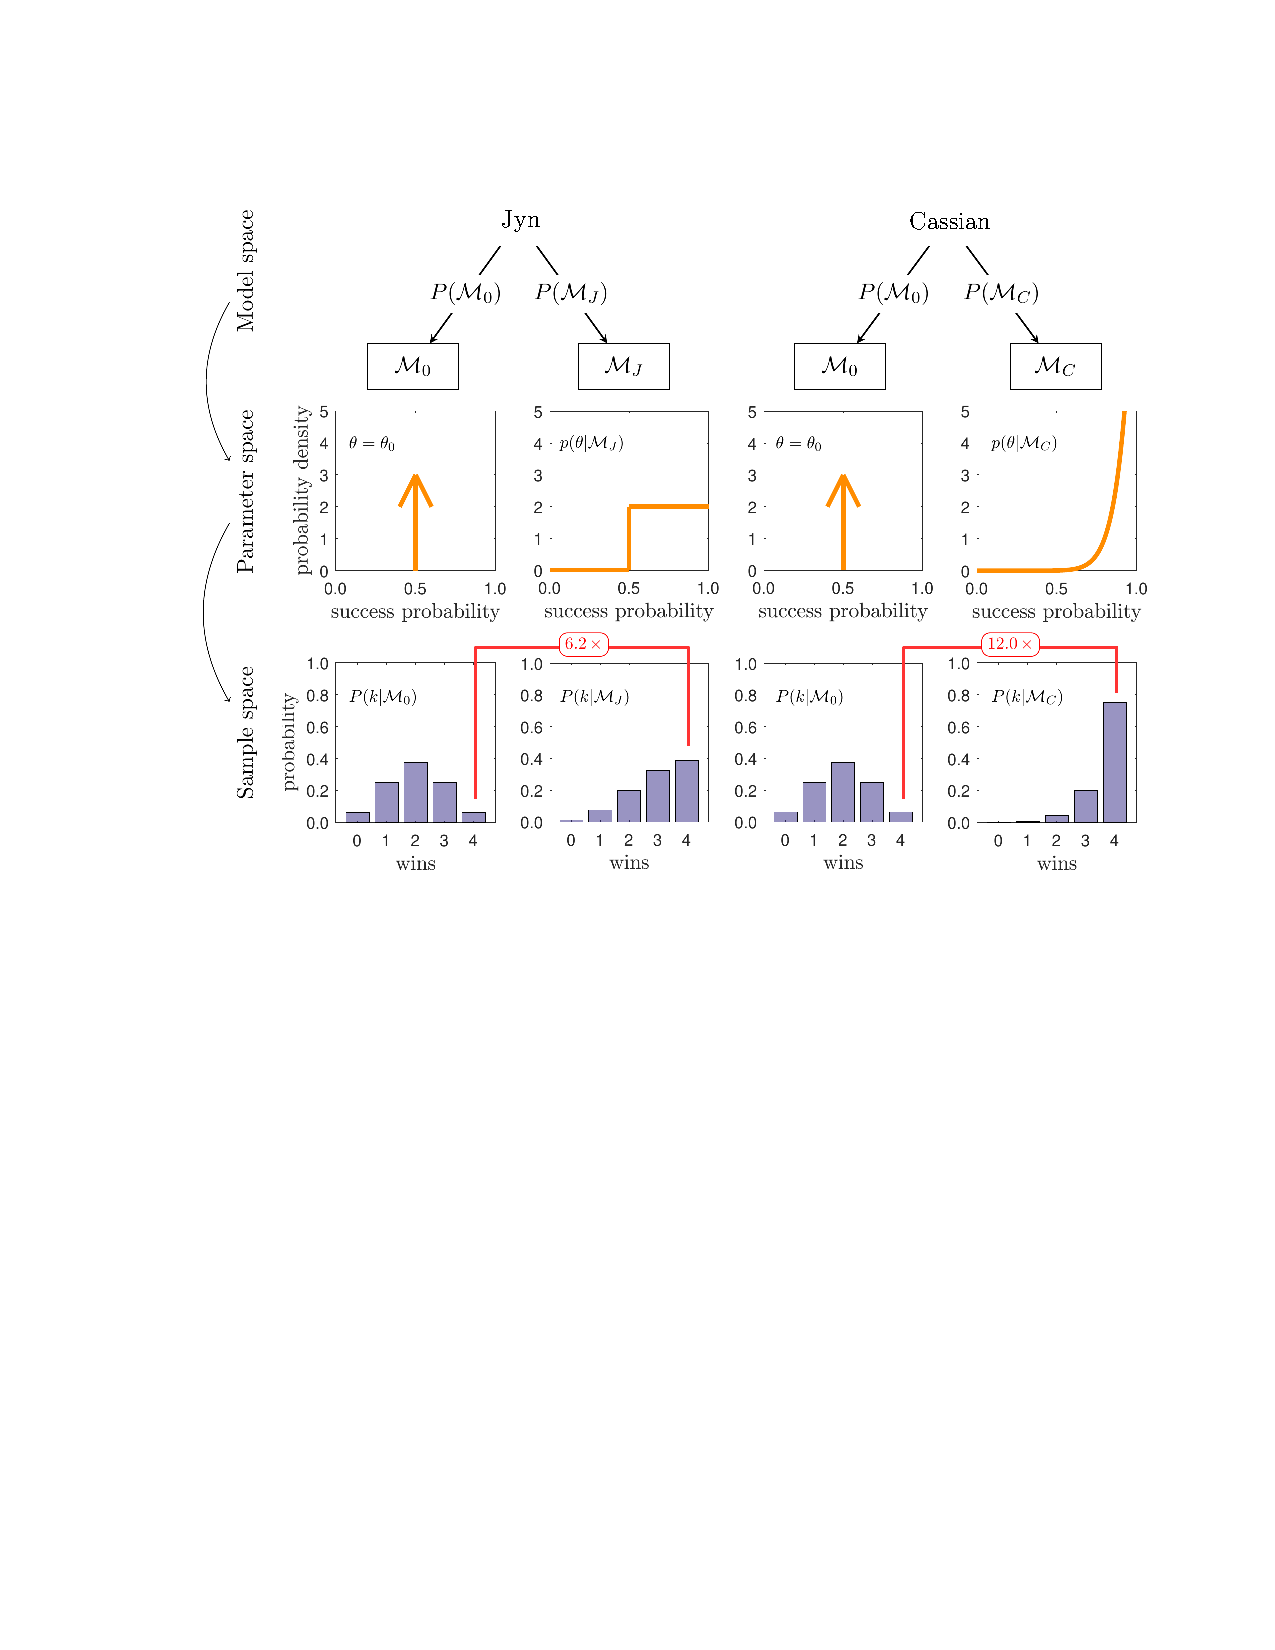
\includegraphics[scale=1,viewport=97 374 550 697]{figs/starwars_fig7.pdf} \vspace{2ex}
\caption{The structure of Jyn and Cassian's models, which can be viewed as more complex (rotated) versions of earlier path diagrams. \textbf{Top:} The model space shows the contending models. In this case, both Jyn and Cassian are comparing two models. The prior probabilities for the models are left unspecified. \textbf{Middle:} The parameter space shows what each model predicts about the true value of $\theta$ (i.e., each model's \textit{conditional prior distribution}). Jyn and Cassian both use a point null model, which packs all of its mass into a single point (shown as the arrow spiking at $\theta=.5$). However, they have different background knowledge about the \textit{midi-chlorian concentrate}, so their prior distributions for $\theta$ under their respective alternative model differ. Note that $p(\theta|M_C)$ is obtained from updating $p(\theta|M_J)$ with 11 additional concentrate-assisted successes. \textbf{Bottom:} The sample space shows what each model predicts about the data to be observed (i.e., each model's prior predictive distribution). The Bayes factor is formed by taking the ratio of the probability each model attached to the observed data, which was four wins in four chance cube tosses. Since the predictions from the null model are identical for Cassian and Jyn, the difference in their Bayes factors is due to the higher marginal likelihood Cassian's alternative model placed on the Naboo captain winning all four chance cube tosses.}
\label{fig:hier}
\end{center}
\end{figure*} 

\paragraph{Example~7b: ``The posterior strikes back''} \label{ex:posterior}
As might be expected, the Naboo grav-ball controversy did not fail to pique interest throughout the galaxy. Independently of the Games Commission statistician, Cassian Andor, Editor-in-Chief of an underground Rebel HoloNet bulletin, had noticed the same peculiar luck in the Naboo team's pregame tosses. In the editor's case, however, attention to the chance cubes was not a coincidence -- in fact, illicit Force enhancement had helped him win a few career-saving tosses in a mildly embarrassing part of his journalistic past.

Cassian's experience with the \emph{midi-chlorian concentrate} is straightforward: on eleven different occasions did he take the serum just before a chance cube toss would decide which of two journalistic leads he would pursue that day -- his colleague would pursue the other. He recalls clearly that on each of the eleven occasions, his leads carried him into the thick of dramatic, newsworthy events while his colleague's leads turned out dead ends. Cassian was promoted; his colleague dismissed.

As it happens, Cassian is an accomplished statistician, and he reasons in much the same way as Jyn (the junior statistician at the Games Commission). If there is no cheating the winning probability should be 50\% each time ($\H_0: \theta = 0.5$). If there \emph{is} cheating, the winning probability should be higher. In contrast to Jyn, however, Cassian has a good idea how much higher the winning probability $\theta$ will be with \emph{midi-chlorian concentrate}: before evaluating the Naboo captain's luck he can estimate $\theta$ from additional information $y$ that only he possesses.

Cassian starts by writing down Equation~\ref{eq:bayesrule3} and filling in the quantities on the right hand side. Among these is the prior density $p(\theta)$, which gives the density at each possible value of $\theta$ \emph{before considering his own eleven winning chance cube tosses $y$}. A reasonable place to start (as before) is that all values between $0.5$ and $1.0$ are equally plausible: $p(\theta) = 2I(0.5<\theta<1.0) = 2I_\theta$ (where we introduce $I_\theta$ as a shorthand for $I(0.5<\theta<1.0)$, the appropriate indicator function). He also uses the same binomial likelihood function as Jyn, hence,
\begin{eqnarray*}
 p(\theta|y) &=& \frac{p(\theta) \times p(y|\theta)}{\int_{\Theta}p(\theta) \times p(y|\theta)d\theta}\\
             &=& \frac{2I_\theta \times \binom{11}{11}\theta^{11}(1-\theta)^0}{\int_{\Theta}2I_\theta \times \binom{11}{11}\theta^{11}(1-\theta)^0d\theta}
              = \frac{2I_\theta \times\theta^{11}}{2\int_{0.5}^{1.0} \theta^{11} d\theta}\\
             &=& \frac{I_\theta \times\theta^{11}}{\left[\frac{\theta^{12}}{12}\right]_{0.5}^{1.0}} = \frac{I_\theta \times\theta^{11}}{\frac{1}{12}\left(1.0^{12} - 0.5^{12}\right)}
         \approx 12\theta^{11}I_\theta.
\end{eqnarray*}

This calculation\footnote{Note that here and below, we make use of a convenient approximation: $0.5^k \approx 0$ for large values of $k$. Making the calculation exact is not difficult but requires a rather unpleasant amount of space. Also note that the indicator function from the prior density carries over to the posterior density.} yields Cassian's \emph{posterior density} of the winning probability $\theta$, which captures his knowledge and uncertainty of the value of $\theta$ under Force doping. The shape of this density function is depicted in the right half of Figure~\ref{fig:hier}. Crucially, Cassian can use this knowledge to perform the same analysis as the Games Commission statistician with only one difference: \textbf{yesterday's posterior $p(\theta|y)$ is today's prior $p(\theta|\H_C)$}. The fact that the latter notation of the prior does not include mention of $y$ serves to illustrate that densities and probabilities are often implicitly conditional on (sometimes informal) background knowledge. Note, for instance, that the entire calculation above assumes that \emph{midi-chlorian concentrate} was taken, but this is not made explicit in the mathematical notation.

Unknowingly repeating Jyn's calculation, Cassian finds that the probability of the Naboo team captain's $k=4$ winning chance cube tosses assuming no Force doping is again $p(k|\H_0) = 1/16$. His calculation for the probability of the $k=4$ wins assuming Force doping is
\begin{eqnarray*}
 P(k|\H_C) &=& \int_{\Theta} p(\theta|\H_C)\times p(k|\theta,\H_C) d \theta \\
     &\approx& \int_{0.5}^{1.0} 12\theta^{11}I_\theta \times \binom{4}{4} \theta^4 \left(1-\theta\right)^0 d \theta \\
           &=& 12 \left[\frac{\theta^{16}}{16} \right]_{0.5}^{1.0}
            = \frac{12}{16} \left(1^{16} - 0.5^{16} \right)
      \approx \frac{12}{16}.
\end{eqnarray*}
To complete his analysis, Cassian takes the ratio of marginal likelihoods, $BF_{C0}=P(k|\H_C)/P(k|\H_0) \approx 12$, which is strong---but not very strong---evidence in favor of the Force-doping model.

Inspired partly by the evidence and partly by the recklessness that follows from years of \emph{midi-chlorian concentrate} abuse, editor Cassian decides to publish an elaborate expos\'e condemning both the Naboo grav-ball team for cheating and the Galactic Games Commission for failing to act on strong evidence of misconduct.

\paragraph{Discussion} This final, two-part example served mostly to illustrate the effects of prior knowledge on inference. This is somewhat in contrast to Example~\ref{ex:droid}, where the prior information was overwhelmed by the data. In the two scenarios {here,} the Games Commission junior statistician and the HoloNet editor are both evaluating evidence that discriminates between two models. Both consider a ``nil model'' in which all parameters are known (the fairness of a chance cube implies that the parameter $\theta$ must be 0.5), but they critically differ in their definition of the alternative model. The Games Commission statistician, having no particular knowledge of the Force-doping serum, considers all better-than-chance values equally plausible, whereas the HoloNet editor can quantify and insert relevant prior information that specifies the expected effects of the drug in question to greater precision.

As illustrated in the bottom row of Figure~\ref{fig:hier}, these three models (the chance model $\H_0$, Jyn's model $\H_J$, and Cassian's model $\H_C$) make distinct predictions: $\H_0$ predicts a distribution of Naboo toss wins that is symmetric about $k=2$; $\H_J$ predicts a right-leaning distribution with a greater probability of four Naboo wins; and $\H_C$ predicts an even greater such probability. More specifically, the marginal likelihoods are $P(k|\H_0) =  5/80$, $P(k|\H_J) = 31/80$, and $P(k|\H_C) \approx 60/80$, and the Bayes factor between any two of these models is given by forming the appropriate ratio.

This example illustrates a general property in Bayesian model comparison: A model that makes precise predictions can be confirmed to a much stronger extent than a model that makes vague predictions, while at the same time the precision of its predictions makes it easier to disconfirm. The reason Cassian was able to obtain a higher Bayes factor than Jyn is because his alternative model made much more precise predictions; $\H_C$ packed three-quarters of its prior predictive distribution into $k=4$, whereas $\H_J$ spread its probability more broadly among the potential outcomes. Since Cassian's precise prediction was correct, he was rewarded with a larger Bayes factor. However, Cassian's prediction was risky: if the Naboo captain had won any fewer than all four tosses, $\H_0$ would have been supported over $\H_C$. In contrast, the Bayes factor would still favor $\H_J$ when $k=3$ because Jyn's model is more conservative in its predictions. In sum, the ability to incorporate meaningful theoretical information in the form of a prior distribution allows for more informed predictions and hence more efficient inferences \cite{LeeSI}.

\section*{Broader appeal and advantages of Bayesian inference}
\epigraph{The Bayesian approach is a common sense approach. It is simply a set of techniques for orderly expression and revision of your opinions with due regard for internal consistency among their various aspects and for the data.}{W.~\citeA{EdwardsEtAl1963}}

\noindent In our opinion, the greatest theoretical advantage of Bayesian inference is that it unifies all statistical practices within the consistent formal system of probability theory.  Indeed, the unifying framework of Bayesian inference is so uniquely well-suited for scientific inference that these authors see the two as synonymous. Inference is the process of combining multiple sources of information into one, and the rules for formally combining information derive from two simple rules of probability. Inference can be as straightforward as determining the event of interest (in our notation, usually $\H$ or $\theta$) and the relevant data and then exploring what the sum and product rules tell us about their relationship. 

As we have illustrated, common statistical applications such as parameter estimation and hypothesis testing naturally emerge from the sum and product rules. However, these rules allow us to do much more, such as make precise quantitative predictions about future data. This intuitive way of making predictions can be particularly informative in discussions about what one should expect in future studies -- it is perhaps especially useful for predicting and evaluating the outcome of a replication attempt, since we can derive a set of new predictions after accounting for the results of the original study \cite<e.g.,>{VerhagenWagenmakers2014,WagenmakersEtAlBathinginpress}.

The practical advantages of using probability theory as the basis of scientific and statistical inference are legion. One of the most appealing in our opinion is it allows us to make probabilistic statements about the quantities of actual interest, such as ``There is a 90\% probability the participants are guessing,'' or ``The probability is .5 that the population mean is negative.'' It also allows us to construct hierarchical models that more accurately capture the structure of our data, which often includes modeling theoretically-meaningful variability at the participant, task, item, or stimulus level \cite{GelmanHill2007,LeeWagenmakersBayesBook,Rouder2016hierarch}.

Bayesian inference also gracefully handles so-called \textit{nuisance parameters.} In most of our present examples there has been only a single quantity of interest -- in order to help keep the examples simple and easy to follow. In real applications, however, there are typically many parameters in a statistical model, some of which we care about and some of which we do not. The latter are called nuisance parameters because we have little interest in them: we only estimate them out of necessity. For example, if we were estimating the mean of a normal distribution (as in Example~\ref{ex:offworlder}) and did not know the population standard deviation, then we would have to assign it a prior density, such that the overall prior density would be of the form $p(\mu,\sigma)$; after collecting data $X$, the posterior density would be of the form $p(\mu,\sigma|X)$. Since we are generally only interested in the parameter $\mu$, estimating $\sigma$ out of necessity, $\sigma$ is considered a nuisance parameter. To make inferences about $\mu$ we merely integrate out $\sigma$ from the posterior density using the sum rule: $p(\mu|X)= \int_{\Sigma}p(\mu,\sigma|X)d\sigma$, from which we can do inference about $\mu$. Similarly, in Examples~\ref{ex:prior} and~\ref{ex:prior}b, the exact win rate from a Force-doped chance cube toss is not of primary interest, only whether the chance cube tossed in the four games was plausibly fair or not. Here, the bias parameter of the chance cube can be seen as a nuisance parameter. Dealing with nuisance parameters in a principled way is a unique advantage of the Bayesian framework: except for certain special cases, frequentist inference can become paralyzed by nuisance parameters.

The ability of Bayesian inference to deal with nuisance parameters also allows it to flexibly handle one of the biggest statistical challenges for data analysts: situations in which the assumptions of the statistical model regarding the data are badly violated. For example, one of the most common assumptions violated is that of normality (e.g., due to the presence of many outliers). In technical terms, this means that we may not think the normal likelihood function adequately characterizes the data-generating mechanism for the inference problem at hand. In Bayesian inference the choice of likelihood is important because, as we have seen in the estimation examples above, with even moderate samples sizes the likelihood quickly begins to dominate the prior densities. To resolve this issue a Bayesian can construct two models: one that uses a normal likelihood function (model $\H_N$), and one that uses a likelihood function with wider tails (model $\H_W$), such as a $t$ distribution with few degrees of freedom. After collecting data we then have a posterior distribution for the parameters of interest for each model, $p(\theta|X,\H_N)$ and $p(\theta|X,\H_W)$. If we assign prior probabilities to these two models (we emphasize that a ``model'' consists of both a prior distribution for the parameters and a likelihood function for the data), $P(\H_N)$ and $P(\H_W)$, we can calculate their posterior probabilities $P(\H_N|X)$ and $P(\H_W|X)$. We are then in a position to use the sum rule to marginalize over the different models (as K2SO did with the various prior densities in Example~\ref{ex:droid}), allowing us to find the \textit{model-averaged} posterior density for $\theta$, $$p(\theta|X)= P(\H_N|X)p(\theta|X,\H_N)+P(\H_W|X)p(\theta|X,\H_W).$$

Note that model averaging is in a sense the flip-side of model selection: In model selection, the identity of the model is central while the \textit{model parameters} are sometimes seen as nuisance variables to be integrated away. By contrast, in the previous equation the \textit{model identities} are treated as nuisance variables while the shared model parameters remain central \cite<see>{Roberts1965,EtzOrigin}. The flexibility to perform model averaging across any variable we care to name \cite<e.g.>{HoetingEtAl1999,link2009bayes} is a unique advantage of Bayesian inference.

Finally, Bayesian analysis allows for immense freedom in data collection because it respects the \textit{likelihood principle} \cite{BergerWolpert1988}. The likelihood principle states that the likelihood function of the data contains all of the information relevant to the evaluation of statistical evidence. What this implies is that other properties of the data or experiment that do not factor into the likelihood function are \textit{irrelevant} to the statistical inference based on the data \cite{Lindley1993,Royall1997}. Adherence to the likelihood principle means that one is free to do analyses without needing to adhere to rigid sampling plans, or even have any plan at all \cite{Rouder2014PBR}. Note that we did not consider the sampling plan in any of our examples above, and none of the inferences we made would have changed if we had. Within a Bayesian analysis, ``It is entirely appropriate to collect data until a point has been proven or disproven, or until the data collector runs out of time, money, or patience'' \cite[p.\ 193]{EdwardsEtAl1963}. 

\section*{Conclusion}
\epigraph{[W]e believe that Bayes' theorem is not only useful, but in fact leads to the \emph{only} correct formulas for solving a large number of our cryptanalytic problems.}{F.~T.~\citeA{Leahy1960} [emphasis original]}

\noindent The goal of this introduction has been to familiarize the reader with the fundamental principles of Bayesian inference. Other contributions in this special issue \cite{DienesSI,KruschkeSI2} focus on why and how Bayesian methods are preferable to the methods proposed in the \textit{New Statistics} \cite{Cumming2014}. The Bayesian approach to all inferential problems follows from two simple formal laws: the sum and product rules of probability. Taken together and in their various forms, these two rules make up the entirety of Bayesian inference -- from testing simple hypotheses and estimating parameters, to comparing complex models and producing quantitative predictions.

The Bayesian method is unmatched in its flexibility, is rooted in relatively straightforward calculus, and uniquely allows researchers to make statements about the relative probability of theories and parameters -- and to update those statements with more data. That is, the laws of probability show us how our scientific opinions can evolve to cohere with the results of our empirical investigations. For these reasons, we recommend that social scientists adopt Bayesian methods rather than the \textit{New Statistics}, and we hope that the present introduction will contribute to deterring the field from taking an evolutionary step in the wrong direction. 

\bibliography{includes/references}\null
\newpage

\appendix
\section*{Computer code for ``The measure of a droid''} \label{app:droid}
\lstinputlisting[style=MyR]{code/droid.R} 

\end{document}
